\documentclass{article}

% if you need to pass options to natbib, use, e.g.:
\PassOptionsToPackage{}{natbib}
% before loading neurips_2020

% ready for submission
%\usepackage{neurips_2020}

% to compile a preprint version, e.g., for submission to arXiv, add add the
% [preprint] option:
%\usepackage[preprint]{neurips_2020}

% to compile a camera-ready version, add the [final] option, e.g.:
\usepackage[final]{neurips_2020}
% to avoid loading the natbib package, add option nonatbib:
\usepackage{neurips_2020}
\usepackage[utf8]{inputenc} % allow utf-8 input
\usepackage[T1]{fontenc}    % use 8-bit T1 fonts
\usepackage{hyperref}       % hyperlinks
\usepackage{url}            % simple URL typesetting
\usepackage{booktabs}       % professional-quality tables
\usepackage{amsfonts}       % blackboard math symbols
\usepackage{amsmath}
\usepackage{nicefrac}       % compact symbols for 1/2, etc.
\usepackage{microtype}      % microtypography
\usepackage{url}
\usepackage{textgreek}
\usepackage{amsfonts}
\usepackage{caption, subcaption}
\usepackage[pdftex]{graphicx}

\title{Uncovering the topology of the temporal region in Alzheimer's disease.}

% The \author macro works with any number of authors. There are two commands
% used to separate the names and addresses of multiple authors: \And and \AND.
%
% Using \And between authors leaves it to LaTeX to determine where to break the
% lines. Using \AND forces a line break at that point. So, if LaTeX puts 3 of 4
% authors names on the first line, and the last on the second line, try using
% \AND instead of \And before the third author name.

\author{%
  Philip Hartout\thanks{With thanks to Bastian Rieck for the supervision and Sarah Brueningk, Felix Hensel, Catherine Jutzeler, Merel Kuijs and Louis Lukas for insightful discussions, code, and data.}\\
  Department of Biosystems Science and Engineering\\
  ETH Zürich\\
  Zürich, Switzerland \\
  \texttt{phartout@ethz.ch} \\
}

\begin{document}

\maketitle

\begin{abstract}
Topological data analysis on medical imaging data is an emerging field leveraging the shape of data for machine learning tasks. Here, we apply a topological data analysis pipeline to uncover novel insights in the Alzheimer's disease neuroimaging initiative dataset. First, we apply persistent homology on a patch of the temporal lobe to extract persistence images, which we then use to learn to classify between patients suffering from Alzheimer's disease versus cognitively normal patients. We then highlight the topological heterogeneity of each the diagnostic categories in the dataset using various distance functions on the extracted topological features.  We then use these distance functions to investigate the topological heterogeneity among patients who have a deteriorating cognitive condition versus those who do not.
\end{abstract}

\section{Introduction}

\subsection{Alzheimer's disease}\label{sec:ad_context}

Alzheimer's disease (AD) is the most prevalent form of dementia in the world, with a forecasted 75 million cases in 2030 and 132 million by 2050 \citep{world2017global}. In EU member states and Switzerland, AD is already among the leading causes of death, and is projected to further accelerate in the future \citep{sleeman2019escalating}. The associated costs are immense --- in the United States alone, the cost of care of AD patients is expected to be \$2 trillion by 2030 ---, and is poised to substantially burden the economic prosperity of developed countries in the future ~\citep{world2017global}.

Crucial to the path of finding a working solutions for patients developing Alzheimer's disease is diagnosing the pathology early, so that nerve damage is minimized once treatment has been found ~\citep{yiannopoulou2020current}. Although the definite diagnosis of a patient with Alzheimer's disease can only be done post-mortem, clinicians use a plethora of standardized tools to find indications of the developing pathology as early as possible, ranging from neuropsychological tests, blood and cerebrospinal fluid markers, and MRI images ~\citep{mckhann2011diagnosis, lehmann2016biomarkers, smits2012early}.

All of these techniques rely on early manifestations of the disease. Although there are disputes on the root cause of the disease in the late onset form of Alzheimer's disease \citep{hur2020innate, fulop2018can, tharp2013origins}, there is still wide consensus that the presence of Amyloid \textbeta{} (A\textbeta{}), which stems from cleavage of amyloid precursor protein (APP), together with the aggregation of neurofibrillary tangles, stemming from hyperphosphorylated tau proteins, accumulate in the brain of patients with Alzheimer's disease, and leads to neural cell death ~\citep{da2016insights}. This cellular destruction leads to an cummulative effect: brain atrophy, particularly in brain regions involved in memory formation such as the medial temporal lobe (MTL), which contains the enthorinal cortex, the hippocampus, and the amygdala \citep{goedert2006century}. These changes can be so pronounced that they are observable using structural Magnetic Resonance Imaging (sMRI) ~\citep{frisoni2010clinical}.

Such images provide an extremely rich source of data, which can then be used for various purposes. One of them is classification, which has been shown to successfully discriminate between cognitively normal (CN) versus AD patients using deep learning techniques such as convolutional neural networks ~\citep{wen2020convolutional}. Additionally, this has lead to the identification of multiple regions being affected by the disease, and patterns have emerged as to which groups of regions are affected, leading to the definition of various subtypes of AD ~\citep{poulakis2018heterogeneous}. To gain even finer insights from the fine but observable alterations of brain shape in the context of Alzheimer's disease, the mathematical field of topology, which studies the properties of geometric objects under continuous deformations, such as stretching, twisting, crumpling and bending, which is exactly the type of deformations occurring in the context of Alzheimer's disease.

\subsection{Topology}

Topology has witnessed relentless theoretical progress since Henri Poincaré first addressed topological ideas as a distinct branch of mathematics in his 1895 publication of \textit{Analysis Situs}~\citep{poincare1895analysis, james1999history}. Only recently, however, with the advent of modern computing, has the field of computational topology and topological data analysis (TDA) gained momentum to investigate complex patterns as shapes observed in physics, biology, and beyond~\citep{ghrist2008barcodes, dey1999computational, amezquita2020shape}. While surveying the various applications of computational topology is beyond the scope of this report, we do want to focus on a number of techniques that are paramount to the workflow described in this report: cubical persistence, various vectorized representations of the persistence diagrams obtained from filtered cubical complexes, and the notion of pairwise distance between such representations. Note that we have not an extensive and formal introduction to topology and persistent homology. For such material, we refer to ~\citep{freedman2009algebraic, edelsbrunner2010computational, ghrist2008barcodes}.


\subsubsection{Cubical complexes and persistent homology}

Prior to defining the notion of cubical persistence, \emph{cubical complexes} need to be defined. For that, let us first assign to each elementary non-degenerate interval $[a,a+1]\forall a\in\mathbb{R}$ two degenerate intervals $[a,a]$ and $[a+1,a+1]$. For a $d$-dimensional space, a cube is then defined as a product of $d$ elementary intervals $\Pi_{i=1}^{d}I_i$. The dimension of the cube is then equal to the number of non-degenerate interval in the aforementioned product, such that 0-cubes, 1-cubes, 2-cubes, and 3-cubes correspond to vertices, edges, squares, and 3D cubes, respectively. In this report, the 3D cube corresponds to a given voxel of our sMRI..

A cubical complex $X$ of dimension $d$ is then defined as a finite set of elementary cubes of at most dimension $d$, where $X$ must be closed undertaking faces and intersections, i.e. for any cube in $X$, all of its faces must belong to $X$, and for any two cube in $X$, their intersection is either empty, or there is a common face between them.

Given a topological space $\mathbb{X}$ (in our case, the sMRI voxels), we use a filtering function $f:\mathbb{X}\to\mathbb{R}$, which here corresponds to the pixel density of each voxel, to study the topology of the sublevel sets $\mathbb{X}_t=f^{-1}(-\infty, t]$ of cubical complexes that arise. This is a method to study topological spaces referred to as \emph{persistent homology}. A common representation of the evolution of topological complexes as a function of the value of the filtration function is the \emph{persistence diagram} (PD), which is a multiset of points. For each homological dimension (here, $1,2,3$), we obtain a collection of points, with an associated $x$ and $y$ coordinate which corresponds to the birth and death of a topological feature in homology dimension $n=1,2,3,\ldots$, respectively. We refer to a homological feature as \emph{persistent} if the difference between its birth and death value with respect to the given filtration function is particularly high.


\subsubsection{Persistence images and persistence landscapes}

PDs are endowed with a metric space; the $p$-Wasserstein distances can be computed between any two persistence image, and these metrics are stable under small perturbations of the data. So, it is possible to perform a variety of ML techiques using PDs as a statistic for clustering. However, multiple ML algorithm require more than a metric, and the computation cost of the $p$-Wasserstein distance increases linearly with the number of points in the PD. It is therefore desirable to have a stable, efficient-to-compute, interpretable (with respect to the PD) and tunable mapping from the PD to a vector space in $\mathbb{R}^n$.

One such representation is the \emph{persistence image} (PI) of a PD, which as been proven to be stable upon small perturbations of data while still retaining the underlying features in the data useful for classification ~\citep{adams2017persistence}. Computing the PI from a PD $D$ consists of a two step process. First, the PD is mapped to an integrable function $\rho_D : \mathbb{R}^2\to \mathbb{R}$ called a persistent surface. This surface is a weighted sum of Gaussian distributions, each centered around a point of the PD. The matrix of pixel values can be obtained from the computation of the integration of $\rho_D$ on a grid overlaid on the surface ~\citep{adams2017persistence}.

Another representation associated to the PD is the persistence landscape (PL)~\citep{bubenik2015statistical, bubenik2020persistence}. This representation maps the PD into a Hilbert space, which is useful for ML applications. In order to define a persistence landscape, let us take a pair $(b,d)$, which refer to the birth and death of a feature. We now define the piecewise linear function $f_{(b,d)}:\mathbb{R} \to [0, \infty]$ as
\begin{equation}
  \label{eq:piecewise_linear_landscape}
  f_{(b,d)}(x)=
  \begin{cases}
    0 & \text{if }x \notin (b,d)\\
    x-b & \text{if }x\in (b,{b+d\over 2}]\\
    -x+b & \text{if }x\in ({b+d\over 2},d]
  \end{cases}
\end{equation}

The PL of the birth-death pairs $\left\{b_i,d_i\right\}_{i=1}^{n}$ is the sequence of functions $\lambda_k:\mathbb{R}\to [0,\infty]$, $k=1,2,3,\ldots$ where $\lambda_k(x)$ is the $k^{th}$ largest value of $\left\{f_{b_i, d_i}(x)\right\}^{n}_{i=1}$. We set $\lambda_k(x)=0$ if the $k^{th}$ largest value does not exist, which results in $\lambda_k=0$ for $k>n$. % An example of PL is shown in % figure~\ref{fig:pl_bubenik}.

% \begin{figure}
%   \centering
%   \begin{minipage}{60mm}
%     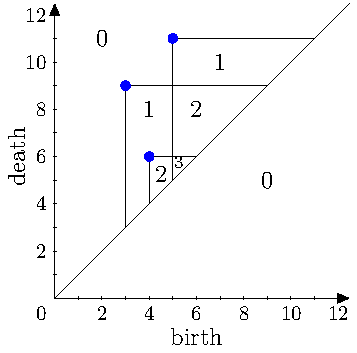
\includegraphics[width=43mm]{figures/persistence_landscape_bubenik_paper/landscapes-figure7.pdf} %     \vspace{1ex}
%     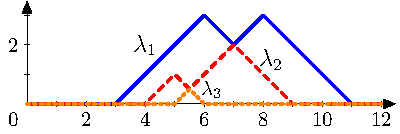
\includegraphics[width=53mm]{figures/persistence_landscape_bubenik_paper/landscapes-figure9.pdf}
%   \end{minipage}
%   \begin{minipage}{60mm}
%     \vspace{5ex}
%     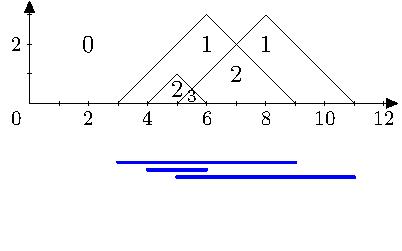
\includegraphics[width=53mm]{figures/persistence_landscape_bubenik_paper/landscapes-figure8.pdf} %     \vspace{-5ex}
%     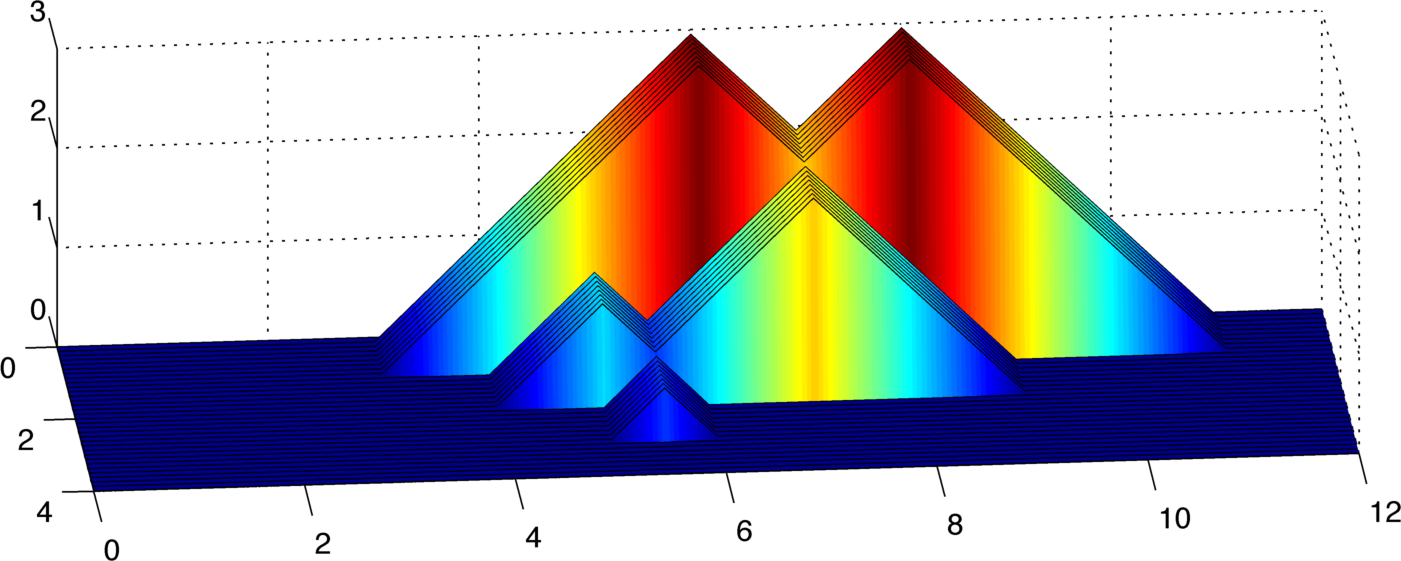
\includegraphics[width=53mm]{figures/persistence_landscape_bubenik_paper/paper3dlandscape.png}
%   \end{minipage}
%   \vspace{5ex}
%   \caption{PL for the homology in degree 1 of linked annuli from %   \citep{bubenik2015statistical}. Top left, persistence diagram, top %   right, rescaled function from equation %   \ref{eq:piecewise_linear_landscape}. Bottom left and right, 2 and 3d %   representation of the persistent landscape. Note that $\lambda_1$ %   represents the most persistent topological features.}
%   \label{fig:pl_bubenik}
% \end{figure}

\subsubsection{Pairwise distances and means}

A crucial element in our investigations is the concept of distance between vectorized topological representations, so let us examine this subject further. Intuitively, and as noted by \citep{berwald2018computing}, it important to take the meaning of the points of the PD into account; namely that a point close to the diagonal $(c,c+\epsilon)$ represents a feature that lived for a short time $\epsilon$. A diagram with this small lifetime point should therefore be close to the same diagram without that point, where the feature would not appear at all. Hence, it makes sense to introduce the notion of minimal cost required to match up points of the two diagrams, either off-diagonal to off-diagonal, or off-diagonal to  the nearest point on the diagonal (for small values of $\epsilon$). In this context, distance functions usually applied to evaluate the distance between two probability density estimations are relevant: the bottleneck distance and the $p$-Wasserstein distance, where $p\geq 1$. The $p$-Wasserstein distance between two diagrams $D_1$ and $D_2$ is the infimum over all bijections $\gamma: D_1 \cup \Delta \to D_2 \cup \Delta$, where $\Delta$ is the multiset $\lbrace (s, s) \mid s \in \mathbb{R} \rbrace$ with multiplicity $(s,s) \mapsto +\infty$, of
\begin{equation}
  \label{eq:wasserstein_distance}
  \left(\sum_{x \in D_1 \cup \Delta} ||x - \gamma(x)||_q^p \right)^{1/p}
\end{equation}

where we usually have $q=\infty$. When we let $p\to\infty$, we recover the bottleneck distance.

We also use the notion of a median persistence landscape, where given a collection of PD, we compute their associated PL, which is a matrix of fixed dimension $m\times h$ where $m$ is the length of the vector, and $h$ is the homology dimension. We compute the average PL by taking the median over all samples for each cell in $m$ for each homology dimension $h$, so we end up with a PL representative of the collection of the samples in the collection.

\subsection{Research questions and outline}

In this report, we answer the following research question: first, how salient are the topological features extracted from the patch for the classification of AD versus CN subjects? Second, how can the distance between any topological representation and the median topological representation of a diagnostic category help us characterize a given diagnostic category? Third, how can the distance among persistent images taken for each patient over the course of the disease inform us with regard to the progression of the patient during the monitoring period?

This report is structured as follows: after having introduced AD and fundamental concepts related to TDA in this introduction, we go on to present and justify methodological choices we have made regarding the topological data analysis conducted on sMRI data in section \ref{sec:methods}; in section \ref{sec:results}, we report the findings extracted from the data, which we discuss in section \ref{sec:discussion}.

\section{Methods}\label{sec:methods}

Here, we present and justify the specific methodological choices made for this pipeline. All of the code used to compute the findings presented in this paper is currently available upon request on \href{https://github.com/pjhartout/TDA_ADNI_MLCB}{GitHub}.

\subsection{Data}

AD and healthy controls of matched age groups (cognitively normal, CN) T1-weighted, 1.5 Tesla sMRIs were obtained from the \href{adni.loni.usc.edu}{Alzheimer's Disease Neuroimaging Initiative} (ADNI) database \citep{jack2008alzheimer}. Further preprocessing steps to reduce noise and extract brains structures is highlighted in appendix \ref{apd:preprocessing}. Then scans were divided into 216 patches, each of dimension ($30\times36\times30$), providing a possibility for a far more focused and computationally efficient investigation while preserving high resolution. In this report, the choice of working with a patch is also supported by the fact that an investigation of \emph{local} changes in brain architecture may reveal more than a brain scan-wide analysis, and has not been performed before.

From earlier work attempting to classify CN subjects from AD patients using a convolutional neural network (CNN), we know that a given patch, shown in grey in figure ~\ref{fig:aucprc}, has a particularly high discriminatory potential, so we selected this patch for all our further analyses. Support for the use of this patch also comes from its anatomical relevance, since it contains regions that are relevant in the context of Alzheimer's disease such as the hippocampus, the enthorinal cortex, and the amygdala ~\citep{goedert2006century}.

\begin{figure}
  \centering
  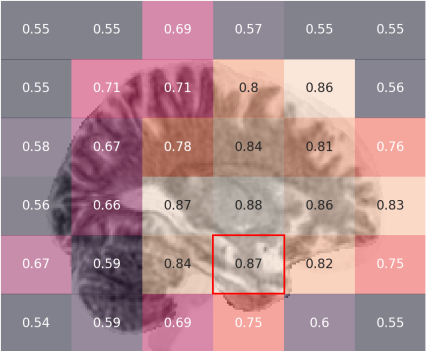
\includegraphics[width=0.4\textwidth]{figures/patch_performance.png}
  \caption{AUCPRC on each patch, achieved using a model described in earlier work. The chosen patch for the topological data analysis is boxed in red.}
  \label{fig:aucprc}
\end{figure}

\subsection{Topological Data Analysis}\label{sec:tda_setup}

To perform the topological analysis on the patch, we used \texttt{giotto-tda}, a library specifically made for the integration of TDA pipelines for ML ~\citep{tauzin2020giottotda}. Each filtration on the cubical complexes has been done in three homological dimensions $1,2,3$, which makes sense given the patch is a three-dimensional image. We otherwise used the default parameters provided by the \href{https://giotto-ai.github.io/gtda-docs/latest/modules/generated/homology/gtda.homology.CubicalPersistence.html#id2}{giotto-tda documentation}.

We also used this library to compute both the persistence images and persistence landscapes. To compute the persistence images, we used 0.05 as a standard deviation for the Gaussian kernel, no weight function, and the default dimension of $100 \times 100$. For the landscapes, we wanted to keep only the most prominent features, so we kept only $\lambda_1$, and set the PL vector lengths of 100.

Computing the average persistence landscape for each diagnostic category was done using the mean of each subject for each of the vector coordinate. The pairwise distance between two PLs was taken using the $L^1$ norm.

Note that we compute the distances in two settings:
\begin{description}
\item[Intra-patient distance]: this allows us to assess the distance of the different PDs of the same patient, to see if there is any evolution over time.
\item[Intra-diagnostic category setting]: here, we compute the
distance of each PL computed from the PD available for a diagnostic category with respect to the mean PL of that image.
\end{description}

\subsection{Model architecture}
For the ML classification task of classifying AD vs CN patients, we used a parallel CNN network, followed by one dense layers containing 500 neurons and with dropout rates of 50\% at training time together. The output of the last dense layer is redirected to a single sigmoid neuron for prediction. The model was trained using an exponential decay learning rate scheduler and early stopping, which monitored the validation loss. All of the layers and utilities to train the neural network were provided by the Keras library ~\citep{chollet2015keras} and are available on the \href{https://github.com/pjhartout/TDA_ADNI_MLCB}{repository}, and a depiction of the computation graph is shown in Figure ~\ref{fig:model_arch}. We also note that the model was trained on commodity hardware, i.e. a Intel(R) Core(TM) i7-9750H CPU @ 2.60GHz for less than a minute per model, highlighting the computational efficiency of the approach.

\begin{figure}
  \centering
  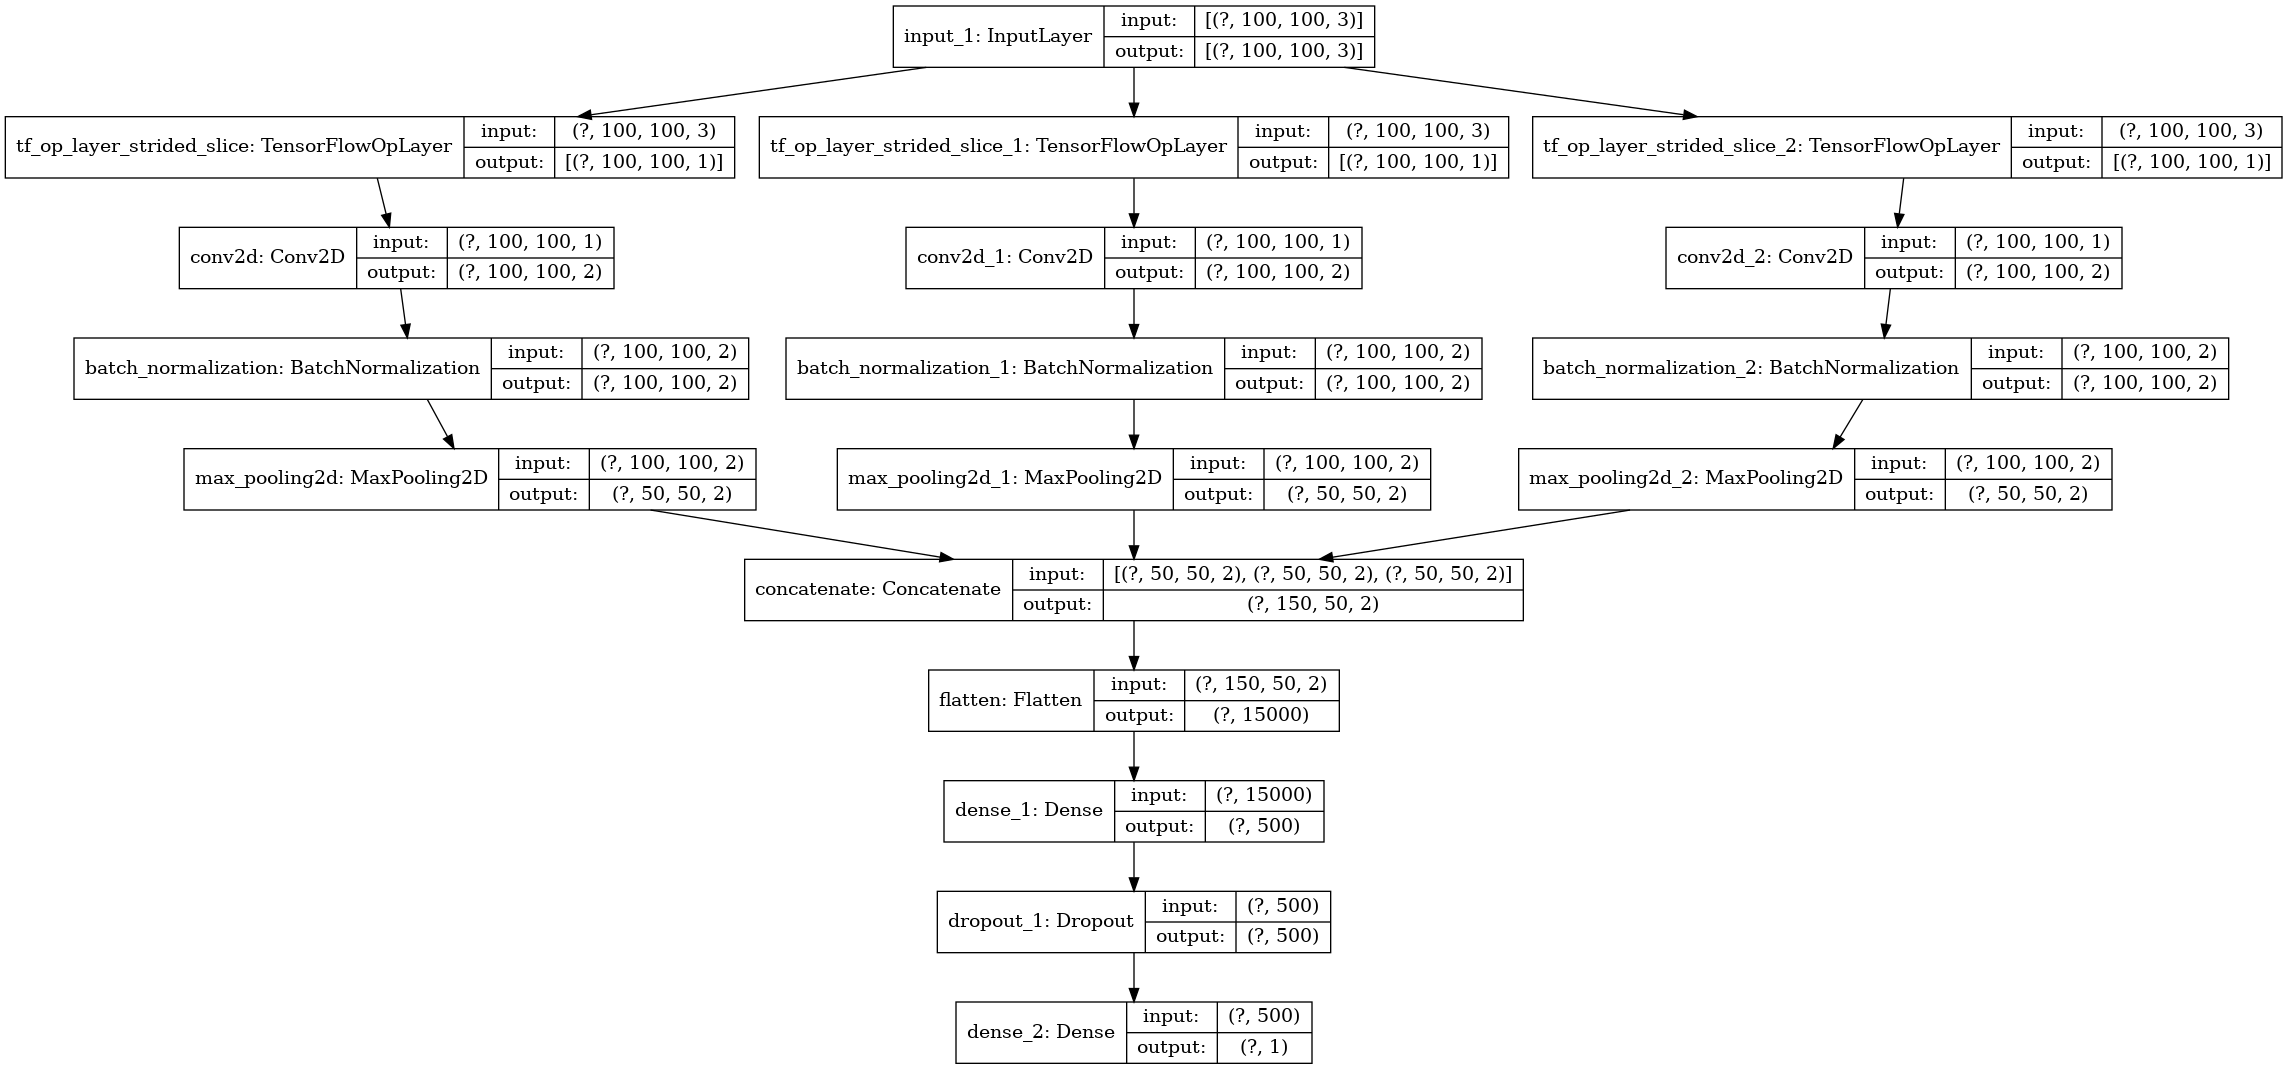
\includegraphics[width=0.9\textwidth]{figures/model.png}
  \caption{Computation graph to predict the phenotype of a given set of persistent images.}
  \label{fig:model_arch}
\end{figure}

\section{Results}\label{sec:results}

Here we present the results obtained from the above-mentioned pipeline, starting with a qualitative assessment of the topological representations obtained from the TDA on the patch from the MTL followed by a performance assessment of the deep learning model. We then turn our attention to the topological heterogeneity observed both within each diagnostic category and then within each patient. Finally, we try to identify patients, so-called topological outliers, which could be potentially misclassified by either the deep learning model or humans.

\subsection{Qualitative assessment of the TDA}

We start by examining an example of the persistence diagram, image and landscape for a randomly sampled CN, MCI, and AD patient, shown in Figure \ref{fig:sample_rep_pd}. No significant difference is immediately apparent from these diagrams, but when we compute their associated PI, we see differences emerging across homological dimensions, as we can observe in Figure \ref{fig:sample_rep_pi}. These differences seem to be salient features in the context of machine learning, should these differences exist in multiple patients.

\begin{figure}
  \centering
  \begin{subfigure}{0.3\textwidth}
    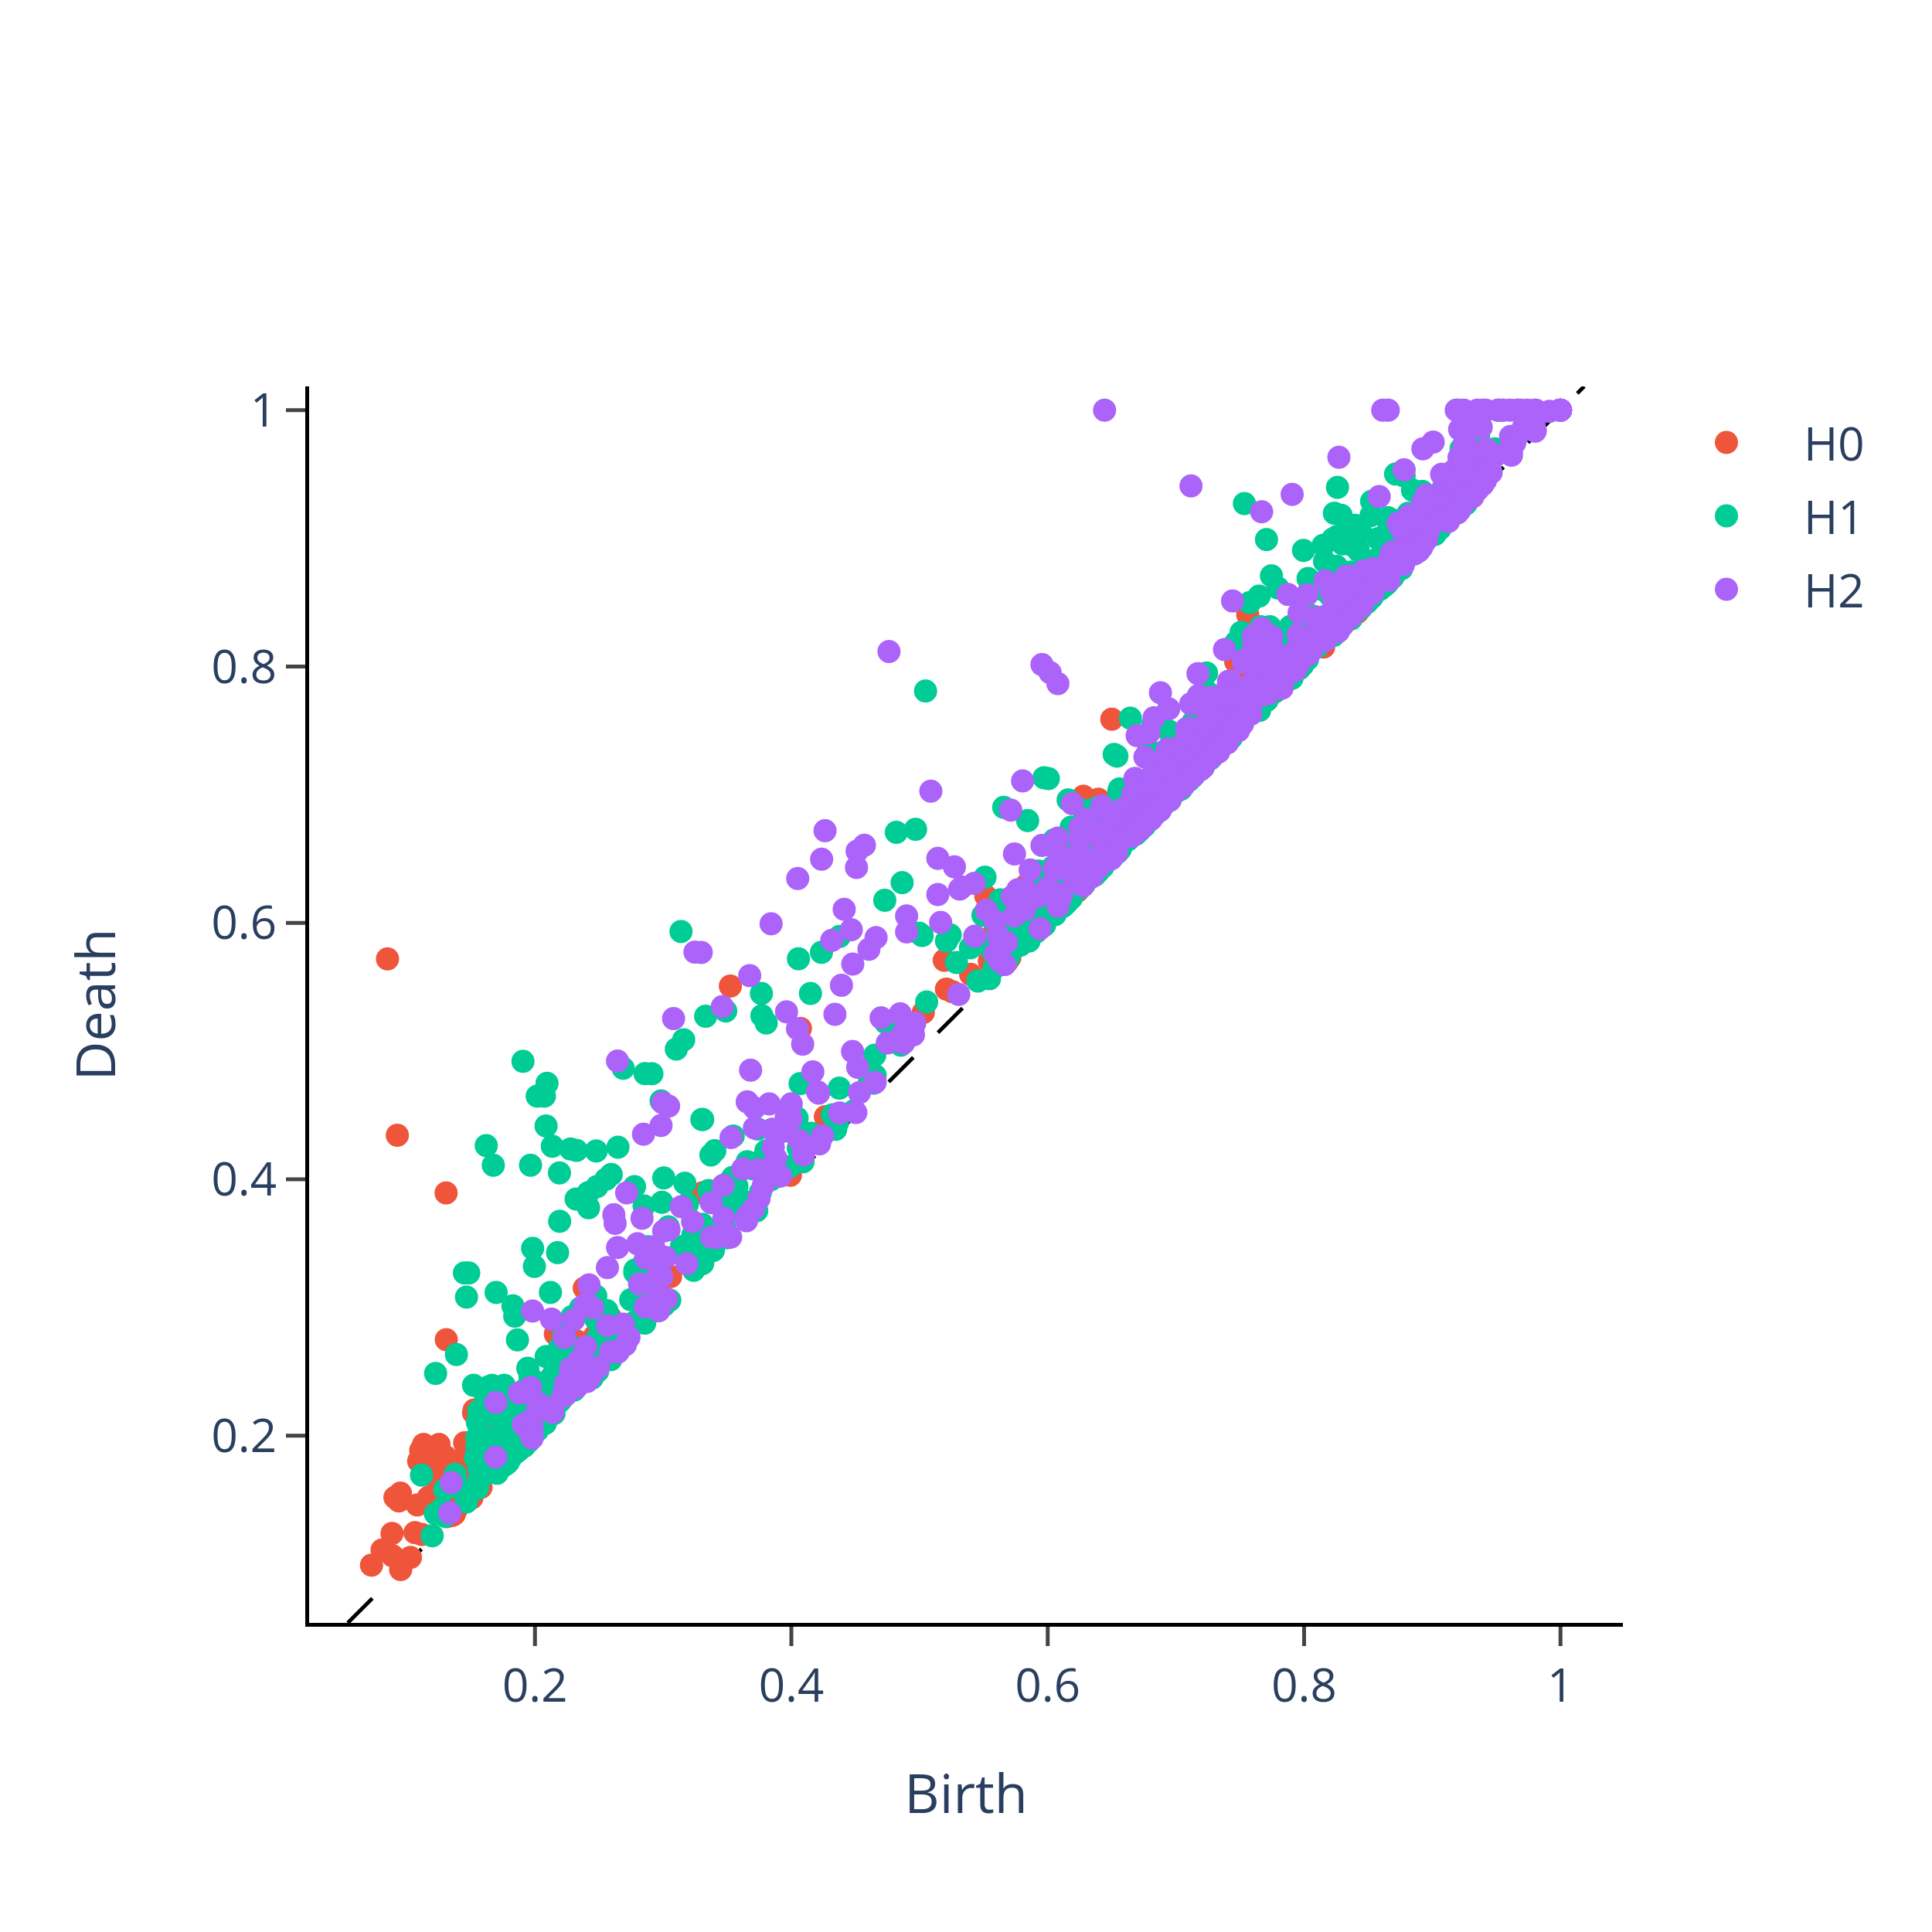
\includegraphics[width=\textwidth]{figures/PDs/persistence_diagram_CN.png}
  \end{subfigure}
  \begin{subfigure}{0.3\textwidth}
    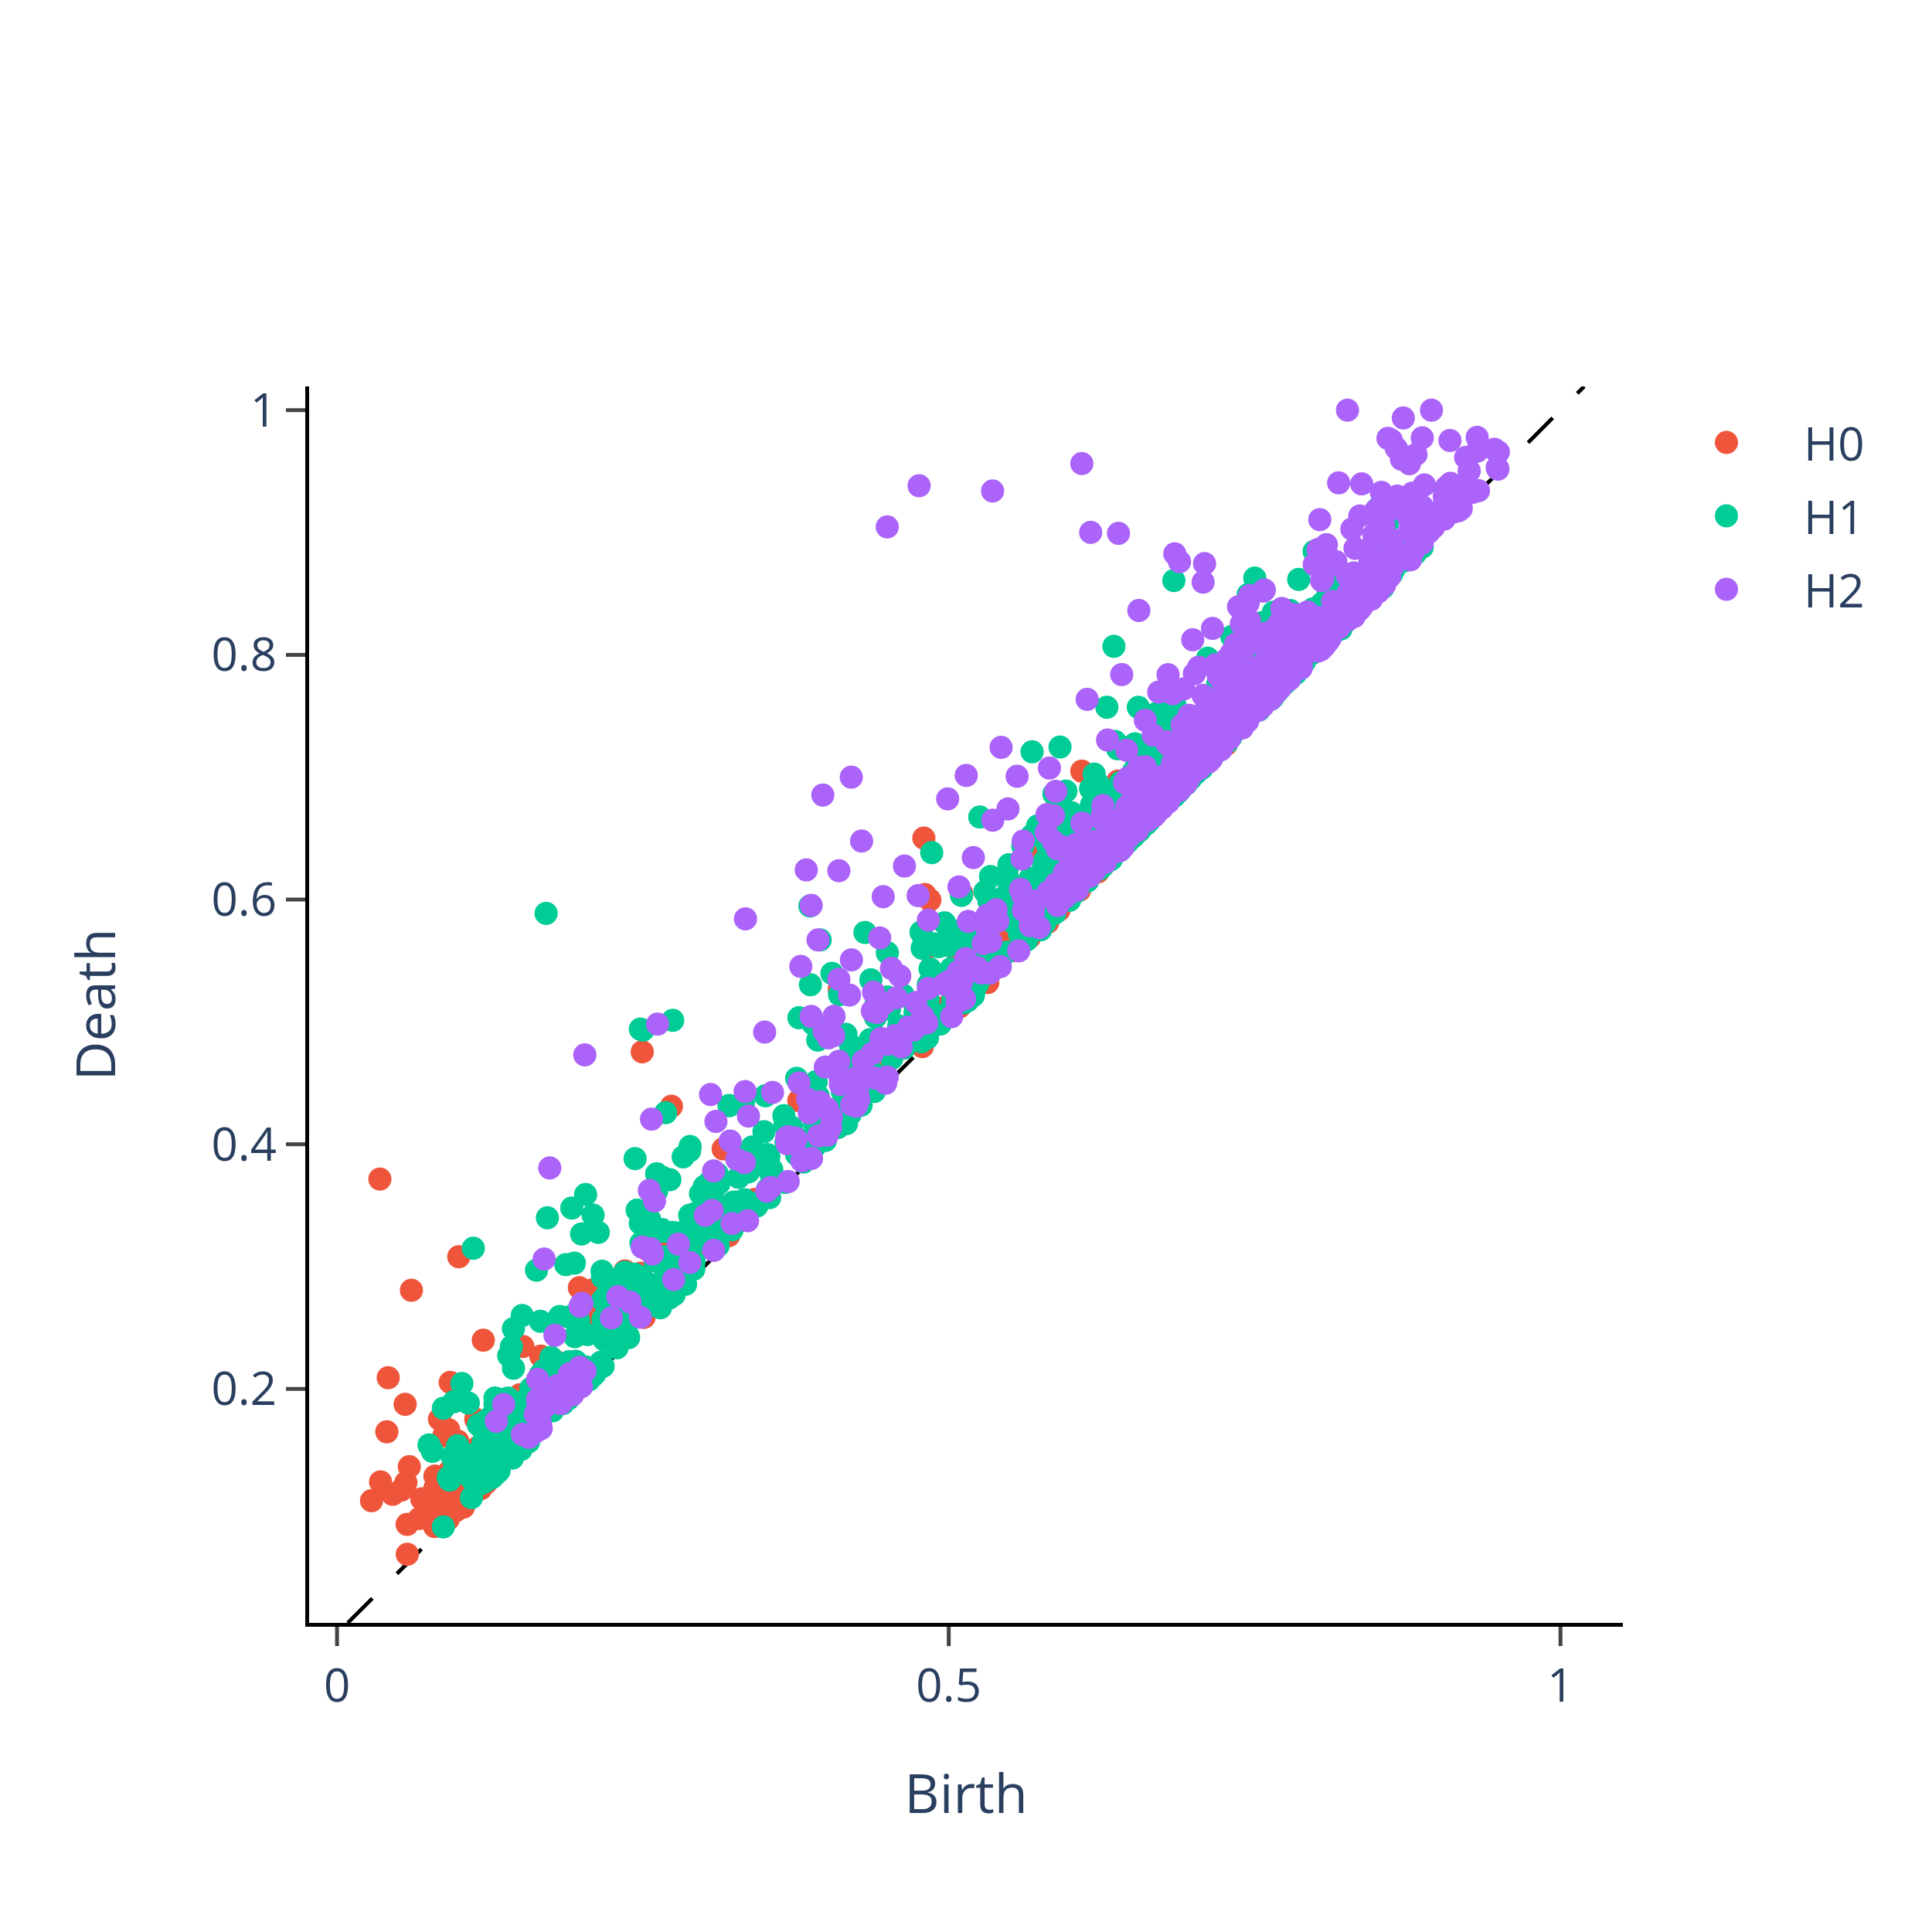
\includegraphics[width=\textwidth]{figures/PDs/persistence_diagram_MCI.png}
  \end{subfigure}
  \begin{subfigure}{0.3\textwidth}
    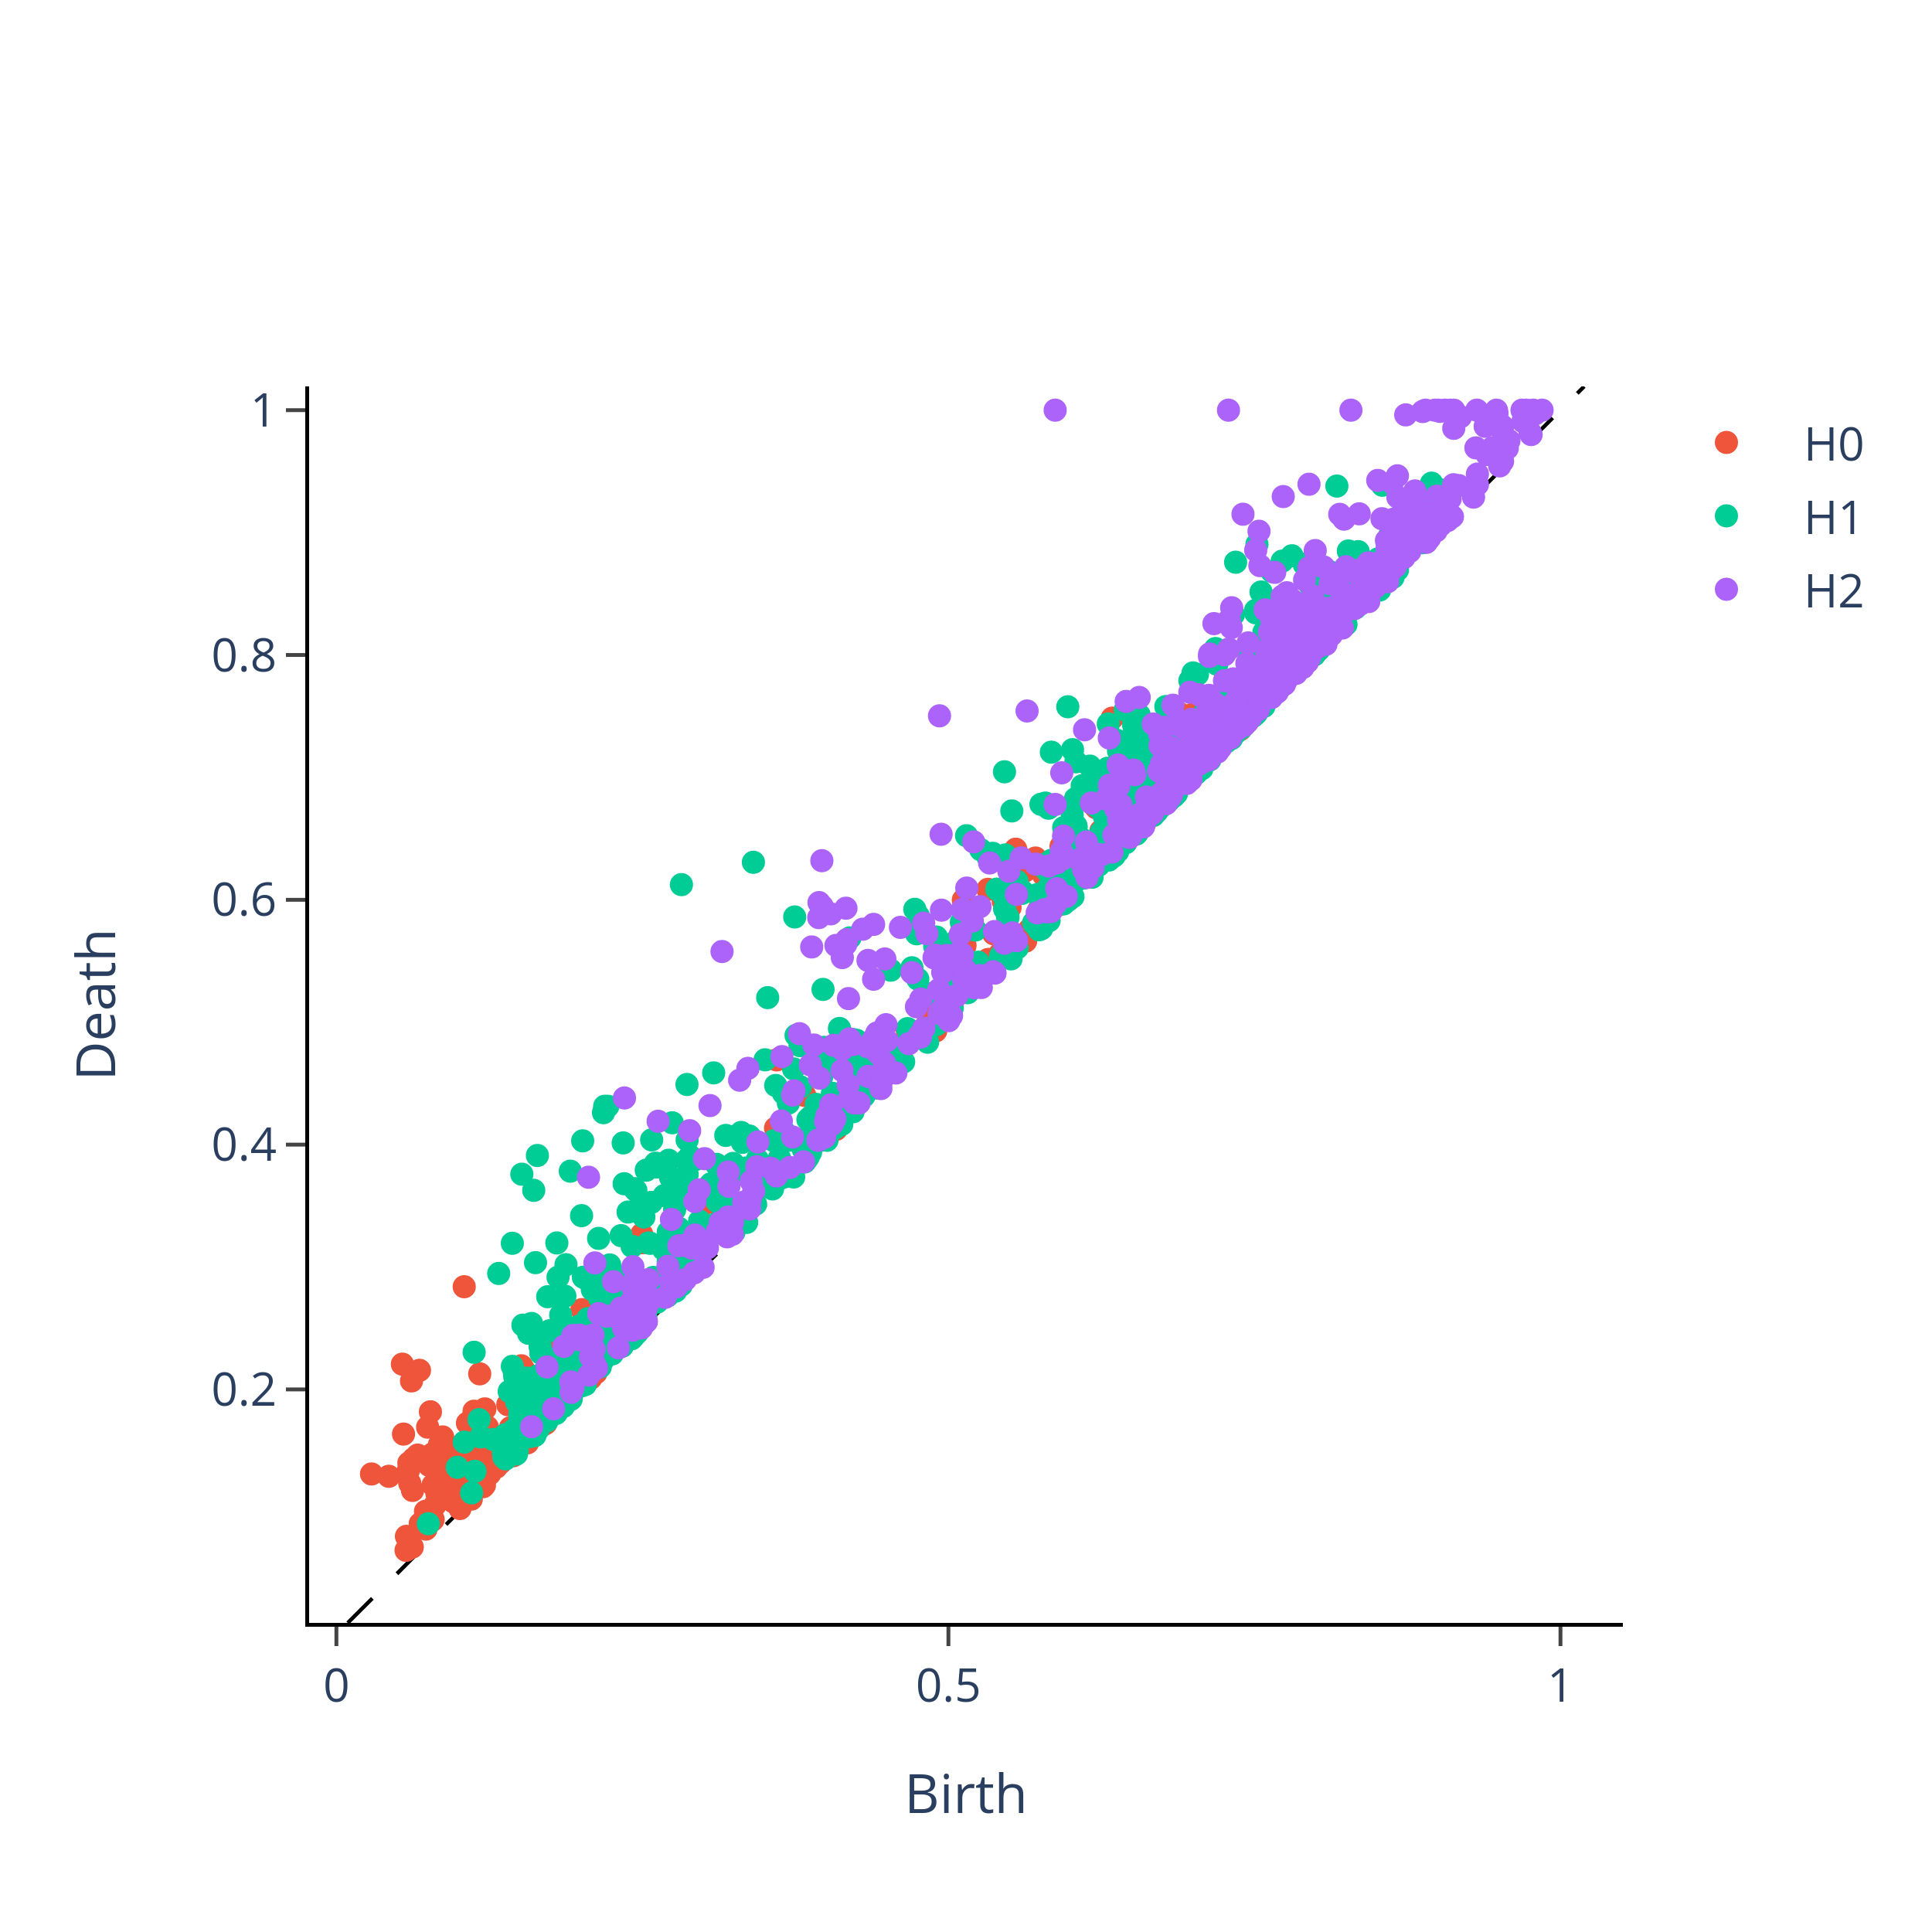
\includegraphics[width=\textwidth]{figures/PDs/persistence_diagram_AD.png}
  \end{subfigure}
  \caption{Representative PD for each of the diagnostic categories.}
  \label{fig:sample_rep_pd}
\end{figure}

\begin{figure}
  \centering
  \begin{subfigure}{0.32\textwidth}
    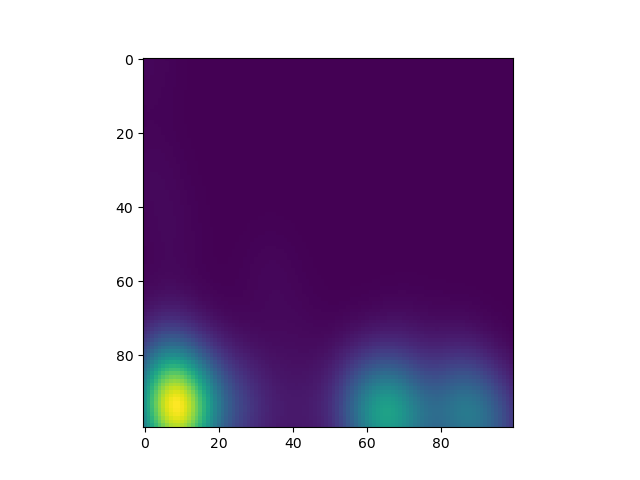
\includegraphics[width=\textwidth]{figures/PIs/Persistence_image_CN_h_0.png}
    \caption{PI of a CN patient in $H_0$}
  \end{subfigure}
  \begin{subfigure}{0.32\textwidth}
    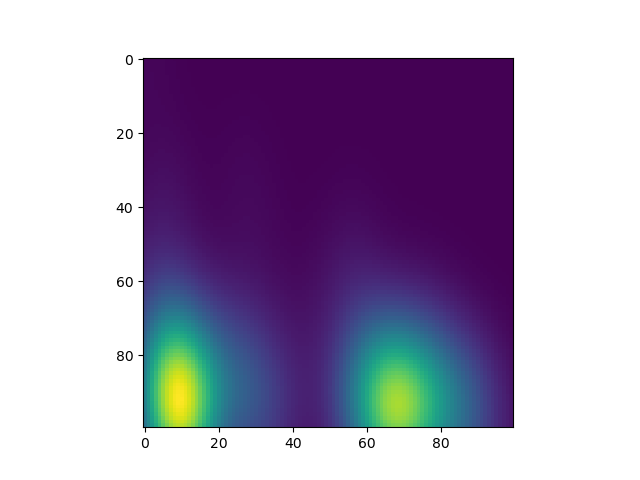
\includegraphics[width=\textwidth]{figures/PIs/Persistence_image_MCI_h_0.png}
    \caption{PI of a MCI patient in $H_0$}
  \end{subfigure}
  \begin{subfigure}{0.32\textwidth}
    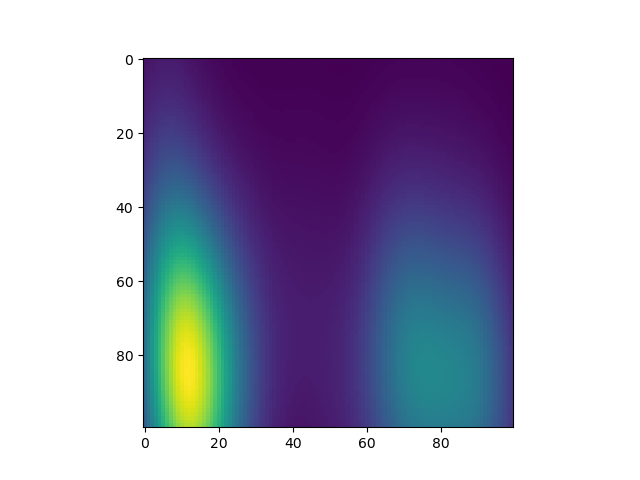
\includegraphics[width=\textwidth]{figures/PIs/Persistence_image_AD_h_0.png}
    \caption{PI of an AD patient in $H_0$}
  \end{subfigure}
  \begin{subfigure}{0.32\textwidth}
    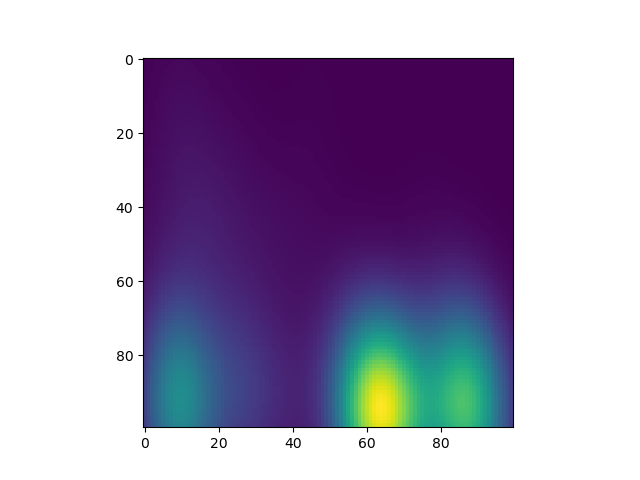
\includegraphics[width=\textwidth]{figures/PIs/Persistence_image_CN_h_1.png}
    \caption{PI of a CN patient in $H_1$}
  \end{subfigure}
  \begin{subfigure}{0.32\textwidth}
    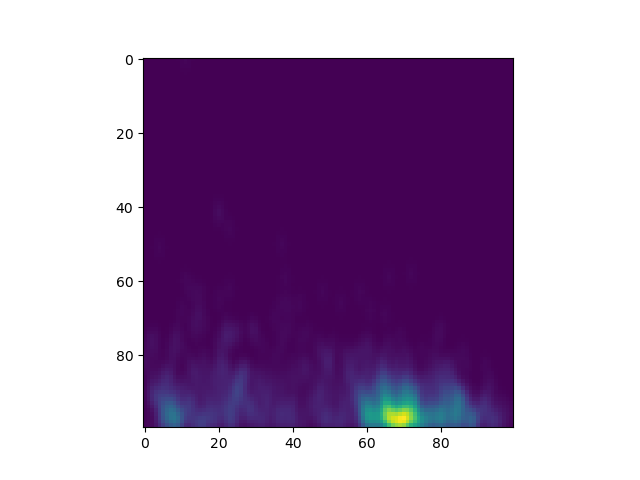
\includegraphics[width=\textwidth]{figures/PIs/Persistence_image_MCI_h_1.png}
    \caption{PI of a MCI patient in $H_1$}
  \end{subfigure}
  \begin{subfigure}{0.32\textwidth}
    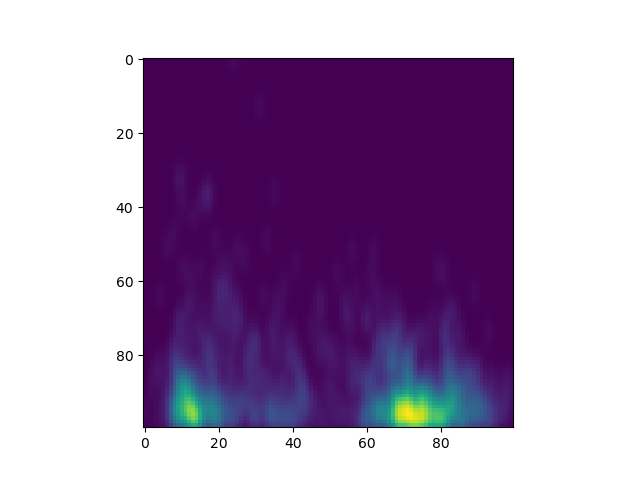
\includegraphics[width=\textwidth]{figures/PIs/Persistence_image_AD_h_1.png}
    \caption{PI of an AD patient in $H_1$}
  \end{subfigure}
  \begin{subfigure}{0.32\textwidth}
    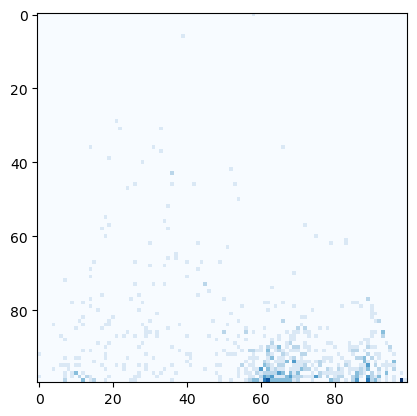
\includegraphics[width=\textwidth]{figures/PIs/Persistence_image_CN_h_2.png}
    \caption{PI of an CN patient in $H_2$}
  \end{subfigure}
  \begin{subfigure}{0.32\textwidth}
    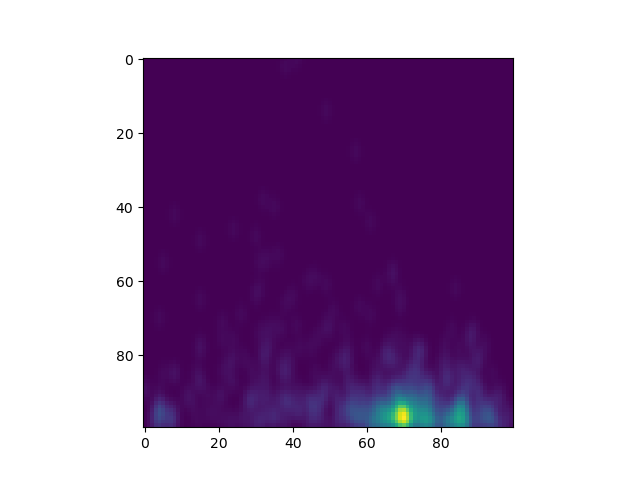
\includegraphics[width=\textwidth]{figures/PIs/Persistence_image_MCI_h_2.png}
    \caption{PI of an MCI patient in $H_2$}
  \end{subfigure}
  \begin{subfigure}{0.32\textwidth}
    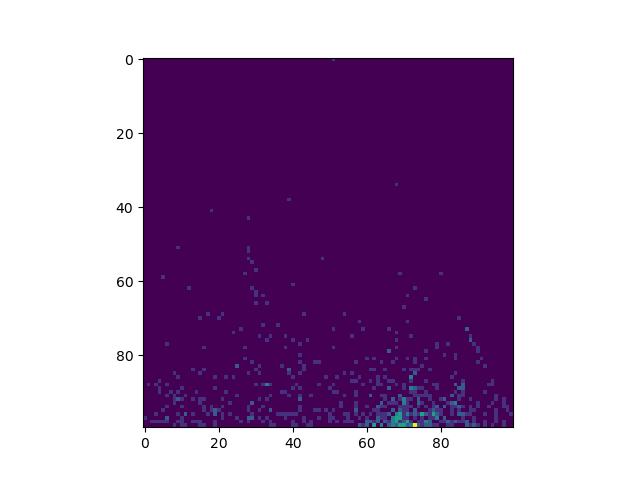
\includegraphics[width=\textwidth]{figures/PIs/Persistence_image_AD_h_2.png}
    \caption{PI of an AD patient in $H_2$}
  \end{subfigure}
  \caption{Representative PI for each of the diagnostic categories. Each column correponds to a diagnostic category whereas each row corresponds to a homological dimension.}
  \label{fig:sample_rep_pi}
\end{figure}

\subsection{Model Performance}

In this report, we trained the deep learning model three times on three different partitions of the data to get an accurate picture of the performance of the model. The performance metrics of the deep learning model is shown in Table ~\ref{tab:performance}. The performance is comparable to state-of-the-art models trained on similar data \citep{wen2020convolutional}.

\begin{table}
  \centering
  \begin{tabular}{lc}
    \toprule
    \textbf{Performance metric} & \textbf{DL model trained on PIs}\\
    \midrule
    Training accuracy & $0.81\pm 0.01$  \\
    Validation accuracy & $0.78\pm 0.03$  \\
    Precision & $0.81\pm 0.04$  \\
    Recall & $0.77\pm 0.03$  \\
    AUC & $0.85\pm 0.03$  \\
    \bottomrule
    \vspace{1pt}
  \end{tabular}
  \caption{Performance metrics of the deep learning model.}
  \label{tab:performance}
\end{table}

\subsection{Topological outliers}

\subsubsection{Between images}

We now present our findings regarding the distribution of the distances between the PL of each image with respect to the median PL for each diagnostic category. The representative PL for each diagnostic category is shown in Figure \ref{fig:median_pls}, and the distribution of the $L^1$ norm between each patient and these median PLs is shown in Figure \ref{fig:displots_median_pl}. As we can see, while the median PLs do not differ too much from one another in each of the homological dimensions, we see that some images seem to have a far greater distance to this median PL than the majority of PLs.

\begin{figure}
  \centering
  \begin{subfigure}{0.32\textwidth}
    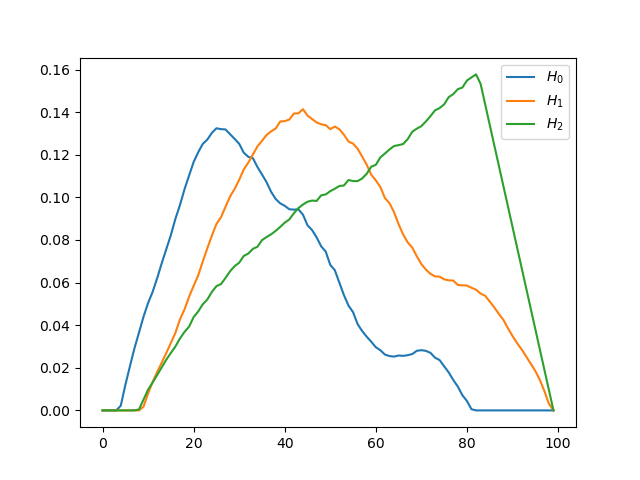
\includegraphics[width=\textwidth]{figures/median_pls/median_pl_CN.png}
    \caption{Median PL for CN subjects}
  \end{subfigure}
  \hfill
  \begin{subfigure}{0.32\textwidth}
    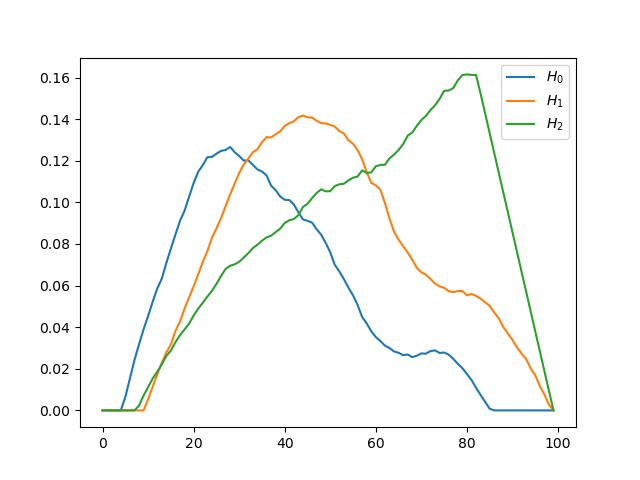
\includegraphics[width=\textwidth]{figures/median_pls/median_pl_MCI.png}
    \caption{Median PL for MCI subjects}
  \end{subfigure}
  \hfill
  \begin{subfigure}{0.32\textwidth}
    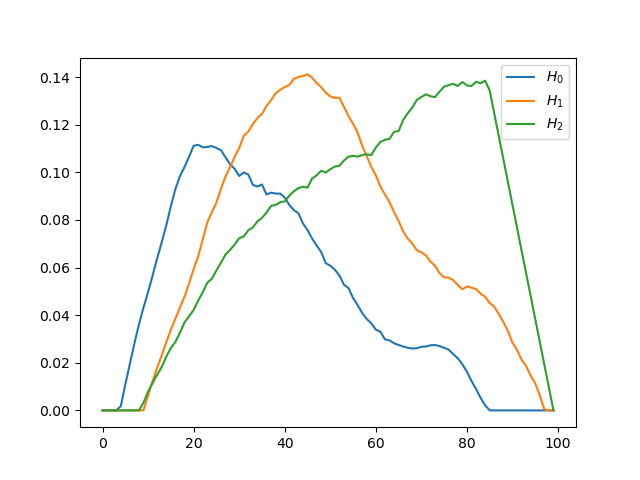
\includegraphics[width=\textwidth]{figures/median_pls/median_pl_AD.png}
    \caption{Median PL for AD subjects}
  \end{subfigure}
  \caption{Median persistence landscapes for each of the diagnostic categories.}
  \label{fig:median_pls}
\end{figure}


\begin{figure}
  \centering
  \begin{subfigure}{0.32\textwidth}
    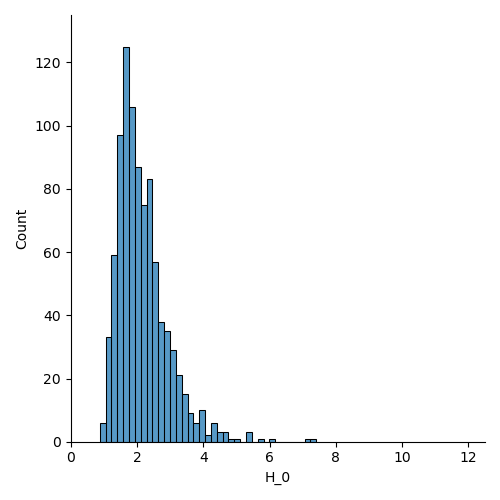
\includegraphics[width=\textwidth]{figures/median_pls/median_pl_CN_H_0.png}
    \caption{$L^1$ norm for CN PLs in $H_0$}
  \end{subfigure}
  \begin{subfigure}{0.32\textwidth}
    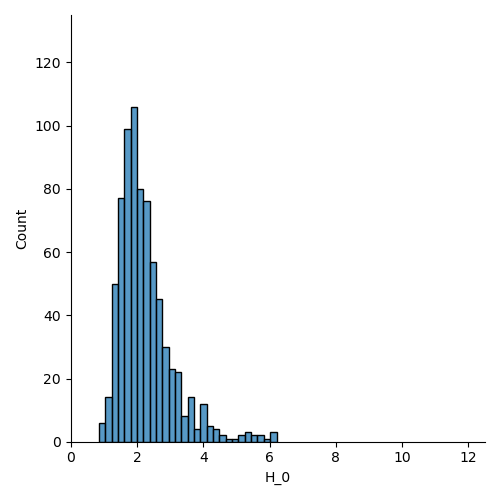
\includegraphics[width=\textwidth]{figures/median_pls/median_pl_MCI_H_0.png}
    \caption{$L^1$ norm for MCI PLs in $H_0$}
  \end{subfigure}
  \begin{subfigure}{0.32\textwidth}
    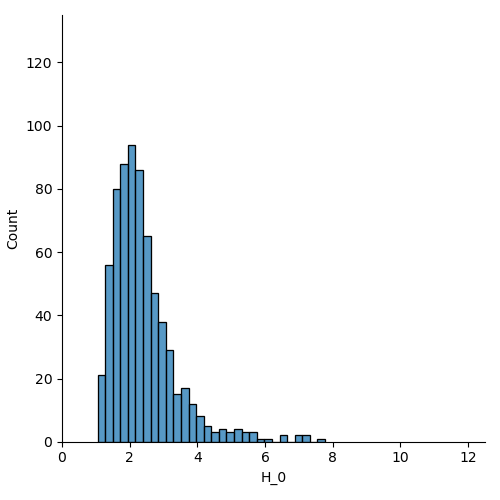
\includegraphics[width=\textwidth]{figures/median_pls/median_pl_AD_H_0.png}
    \caption{$L^1$ norm for AD PLs in $H_0$}
  \end{subfigure}
  \begin{subfigure}{0.32\textwidth}
    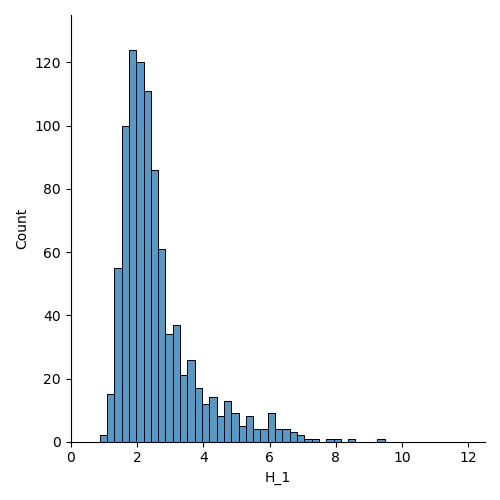
\includegraphics[width=\textwidth]{figures/median_pls/median_pl_CN_H_1.png}
    \caption{$L^1$ norm for CN PLs in $H_1$}
  \end{subfigure}
  \begin{subfigure}{0.32\textwidth}
    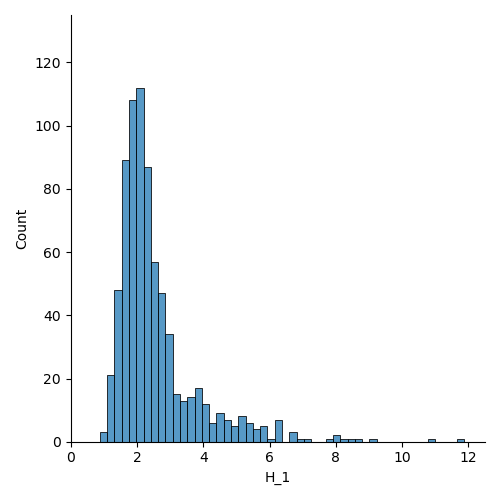
\includegraphics[width=\textwidth]{figures/median_pls/median_pl_MCI_H_1.png}
    \caption{$L^1$ norm for MCI PLs in $H_1$}
  \end{subfigure}
  \begin{subfigure}{0.32\textwidth}
    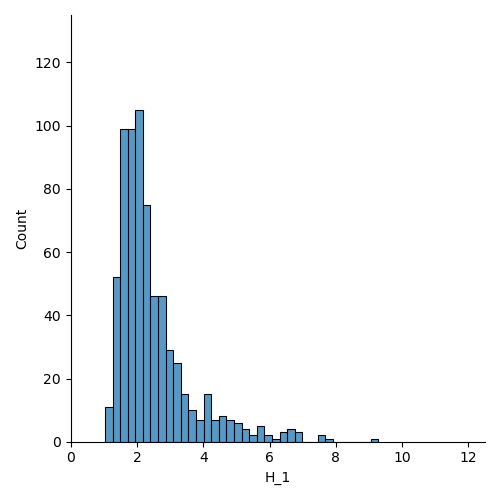
\includegraphics[width=\textwidth]{figures/median_pls/median_pl_AD_H_1.png}
    \caption{$L^1$ norm for AD PLs in $H_1$}
  \end{subfigure}
  \begin{subfigure}{0.32\textwidth}
    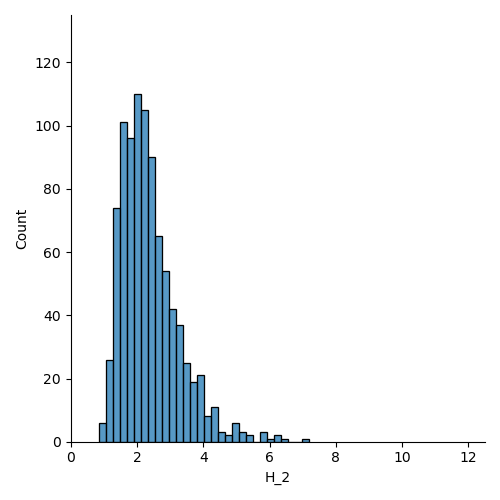
\includegraphics[width=\textwidth]{figures/median_pls/median_pl_CN_H_2.png}
    \caption{$L^1$ norm for CN PLs in $H_2$}
  \end{subfigure}
  \begin{subfigure}{0.32\textwidth}
    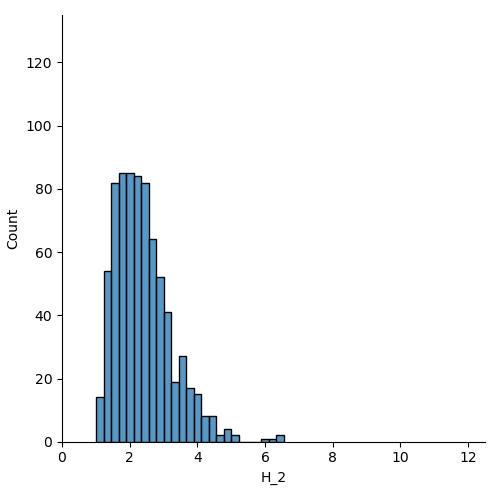
\includegraphics[width=\textwidth]{figures/median_pls/median_pl_MCI_H_2.png}
    \caption{$L^1$ norm for MCI PLs in $H_2$}
  \end{subfigure}
  \begin{subfigure}{0.32\textwidth}
    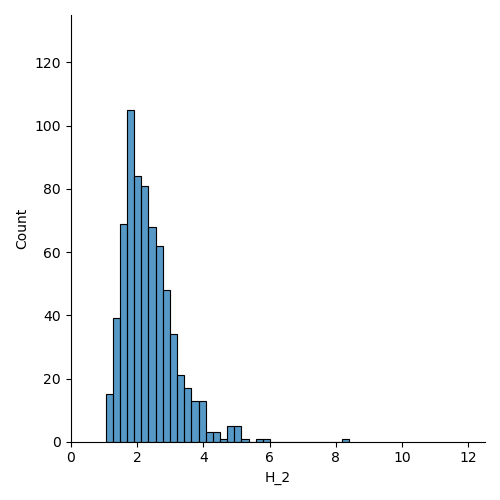
\includegraphics[width=\textwidth]{figures/median_pls/median_pl_AD_H_2.png}
    \caption{$L^1$ norm for AD PLs in $H_2$}
  \end{subfigure}
  \caption{Histogram showing the distribution of the $L^1$ norm taken between the median PL for a diagnostic categories in all homological dimesions.}
  \label{fig:displots_median_pl}
\end{figure}

\begin{table}
\centering
\begin{tabular}{lrrrrrr}
\toprule
{} &  Mean &  Median &  Standard deviation &   Q3 &   Max &  Skewness \\
\midrule
CN $H_0$ & 2.16 & 2.00 & 0.78 & 2.50 & 7.41 & 1.78 \\
CN $H_1$ & 2.61 & 2.27 & 1.17 & 2.93 & 9.47 & 1.92 \\
CN $H_2$ & 2.38 & 2.23 & 0.88 & 2.79 & 7.19 & 1.39 \\
MCI $H_0$ & 2.24 & 2.04 & 0.82 & 2.55 & 6.21 & 1.71 \\
MCI $H_1$ & 2.57 & 2.19 & 1.29 & 2.80 & \textbf{11.87} & \textbf{2.57} \\
MCI $H_2$ & 2.40 & 2.27 & 0.83 & 2.82 & 6.55 & 1.18 \\
AD $H_0$ & 2.40 & 2.18 & 0.96 & 2.77 & 7.77 & 1.97 \\
AD $H_1$ & 2.47 & 2.13 & 1.15 & 2.77 & \textbf{9.28} & \textbf{2.10} \\
AD $H_2$ & 2.36 & 2.20 & 0.80 & 2.75 & 8.39 & 1.64 \\
  \bottomrule
  \vspace{6pt}
\end{tabular}
\caption{Summary statistics of the distribution of distances from median persistence landscapes for each diagnostic category shown in Figure \ref{fig:displots_median_pl}}
\label{tab:stats_median_pl}
\end{table}


\subsubsection{Within patients}

As indicated in section \label{sec:tda_setup}, we can compute the distance between various PLs associated to the different timepoints available to a single patient to evaluate the distance between each of these topological representations at these timepoints, hence obtaining a representation of the topological evolution of that particular patient.

We find interesting qualitative results, with distance varying widely from one patient to the next. For instance, if we take a CN patient diagnosed as such throughout the time that that patient, has been monitored, we see relatively low distances between that patients and other timepoints, see Figure \ref{fig:patient_evolution_stable} for an example. However, this trend drastically changes when taking a patient who transitions from an MCI diagnosis to an AD diagnosis, as can be seen in Figure ~\ref{fig:patient_evolution_mci_ad}. Note that the colorscale is the same for Figures \ref{fig:patient_evolution_stable} and \ref{fig:patient_evolution_mci_ad}. However, these effects do not generalize: if we take the average distance for each homological dimension for each patient and compare the distribution of these averages for patients who deteriorate (i.e. transition from CN to MCI or from MCI to AD) and those who do not, we do not see any quantitative difference, as can be seen in Figure \ref{fig:kde_intra_patient}. Surprisingly, however, we see that taking the average Wasserstein distance for each patient, a bimodal -- similar for both deteriorating and stable patients -- distribution arises, but dissapears as we let $p\to\infty$ as we recover the bottleneck distance. Additionally, while no substantial differences are observes, we do see slight rightwards shifts in each mode for both Wasserstein and the $L^1$ norm of the persistent landscape, indicating a potential shift among some of the observed data points. This is echoed by the fact that the $p$-value computed by the Mann-Whitney $\mathcal{U}$ test are significant for all of these instances.


\begin{figure}
  \centering
  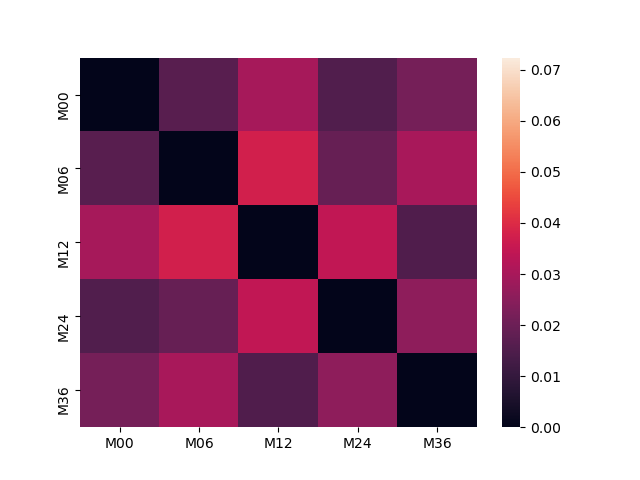
\includegraphics[width=0.32\textwidth]{figures/temporal_evolution/ADNI011S0023_h_0.png}
  \hfill 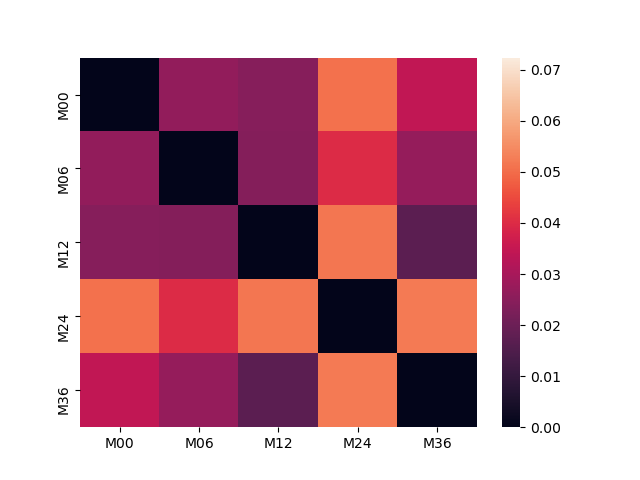
\includegraphics[width=0.32\textwidth]{figures/temporal_evolution/ADNI011S0023_h_1.png}
  \hfill 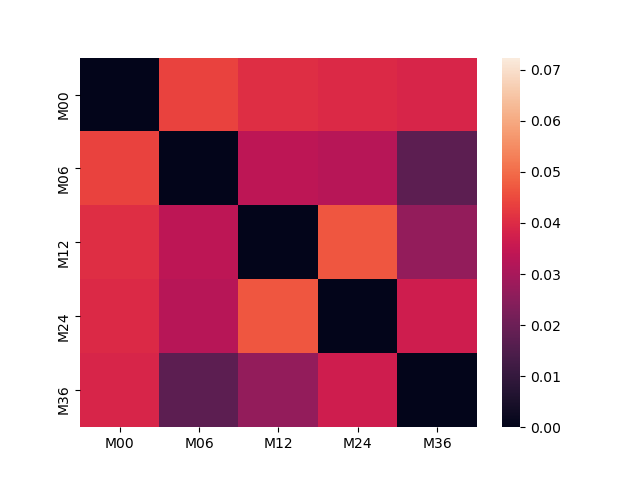
\includegraphics[width=0.32\textwidth]{figures/temporal_evolution/ADNI011S0023_h_2.png}
  \caption{Topological evolution of a subject with an unchanging CN diagnosis.}
  \label{fig:patient_evolution_stable}
\end{figure}

\begin{figure}
  \centering
    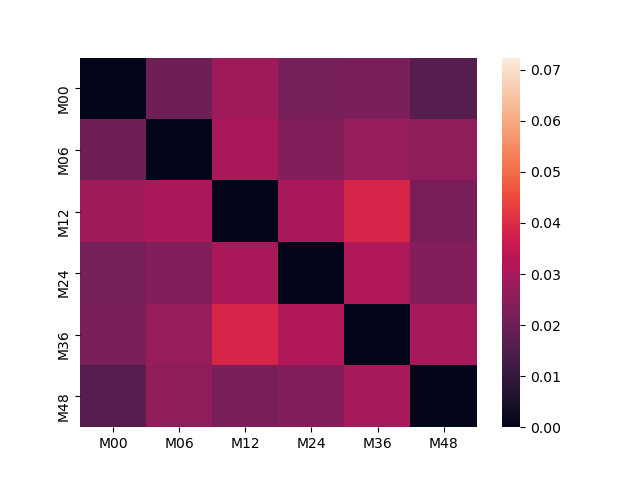
\includegraphics[width=0.32\textwidth]{figures/temporal_evolution/ADNI029S0878_h_0.png}
    \hfill 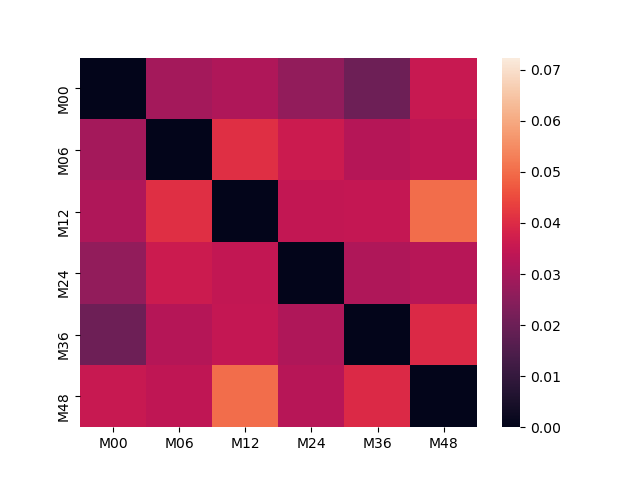
\includegraphics[width=0.32\textwidth]{figures/temporal_evolution/ADNI029S0878_h_1.png}
    \hfill 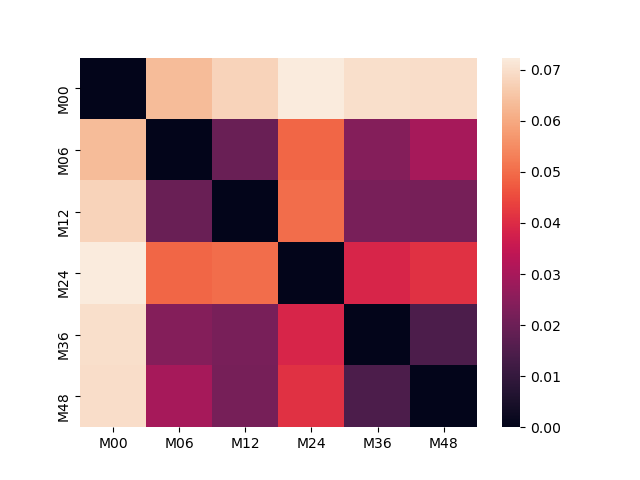
\includegraphics[width=0.32\textwidth]{figures/temporal_evolution/ADNI029S0878_h_2.png}
    \caption{Topological evolution of a patient who transitions from MCI to AD in the course of the observation. For this particular case, the change in diagnosis occurred at $t=24$, i.e. 24 months after the baseline diagnosis, which also corresponds with the highest distance from that baseline.}
    \label{fig:patient_evolution_mci_ad}
\end{figure}


\begin{figure}
  \centering
  \begin{subfigure}{0.32\textwidth}
    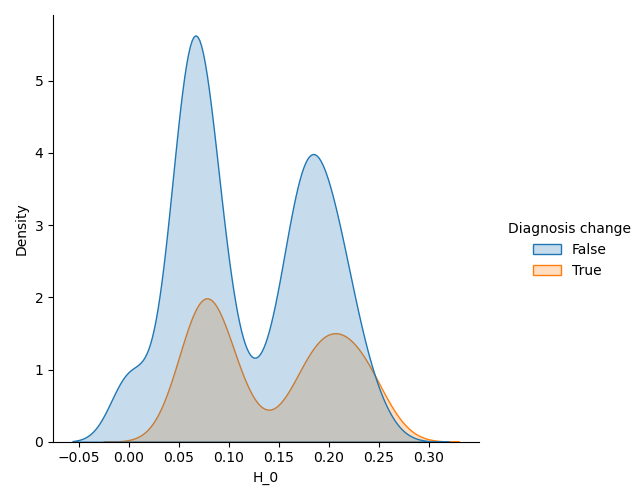
\includegraphics[width=\textwidth]{figures/temporal_evolution/wasserstein_H_0_dist_diag_change.png}
    \caption{Wasserstein distance with $p=2$ in $H_0$}
  \end{subfigure}
  \begin{subfigure}{0.32\textwidth}
    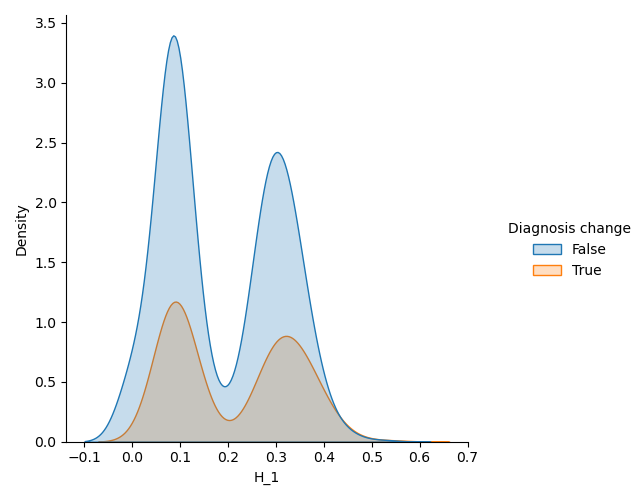
\includegraphics[width=\textwidth]{figures/temporal_evolution/wasserstein_H_1_dist_diag_change.png}
    \caption{Wasserstein distance with $p=2$ in $H_1$}
  \end{subfigure}
  \begin{subfigure}{0.32\textwidth}
    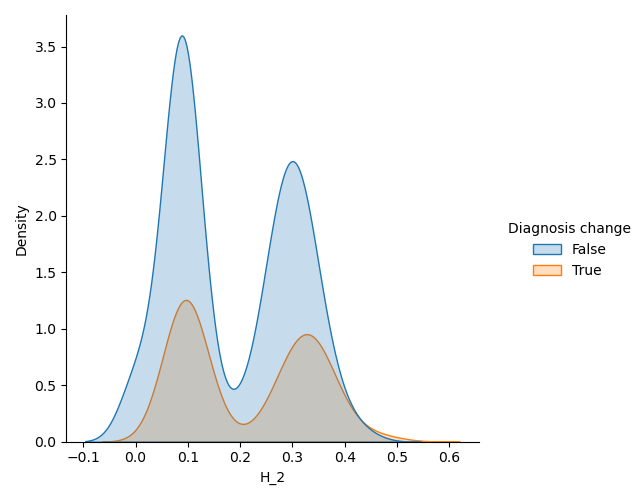
\includegraphics[width=\textwidth]{figures/temporal_evolution/wasserstein_H_2_dist_diag_change.png}
    \caption{Wasserstein distance with $p=2$ in $H_2$}
  \end{subfigure}
  \begin{subfigure}{0.32\textwidth}
    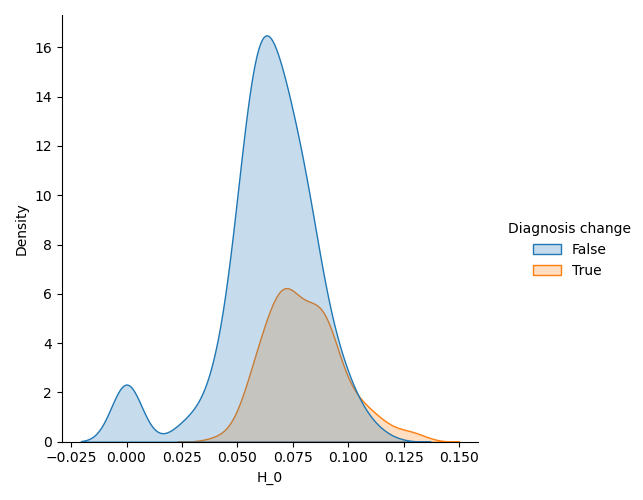
\includegraphics[width=\textwidth]{figures/temporal_evolution/bottleneck_H_0_dist_diag_change.png}
    \caption{Bottleneck distance in $H_0$}
  \end{subfigure}
  \begin{subfigure}{0.32\textwidth}
    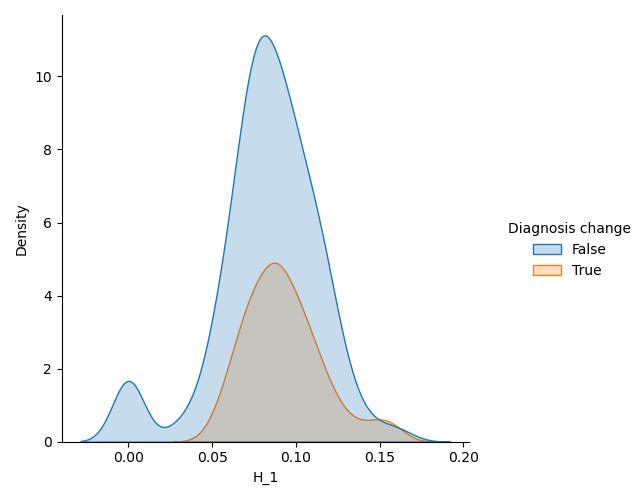
\includegraphics[width=\textwidth]{figures/temporal_evolution/bottleneck_H_1_dist_diag_change.png}
    \caption{Bottleneck distance in $H_1$}
  \end{subfigure}
  \begin{subfigure}{0.32\textwidth}
    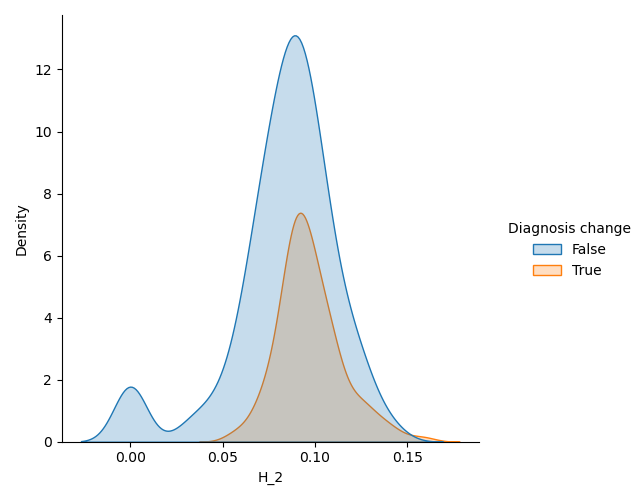
\includegraphics[width=\textwidth]{figures/temporal_evolution/bottleneck_H_2_dist_diag_change.png}
    \caption{Bottleneck distance in $H_2$}
  \end{subfigure}
  \begin{subfigure}{0.32\textwidth}
    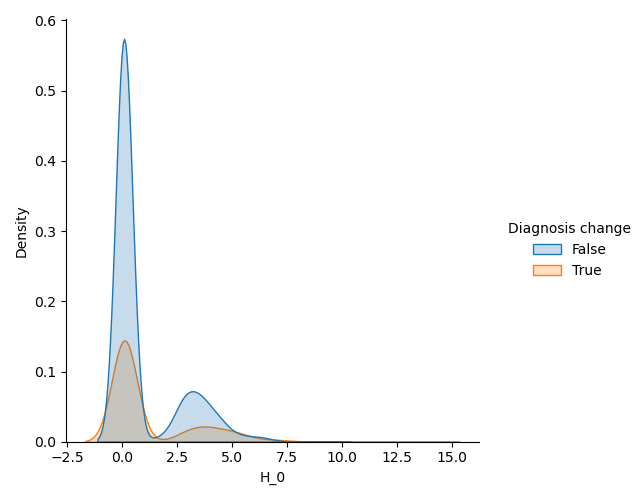
\includegraphics[width=\textwidth]{figures/temporal_evolution/landscape_H_0_dist_diag_change.png}
    \caption{$L^{1}$ landscape distance with 1 layer in $H_0$}
  \end{subfigure}
  \begin{subfigure}{0.32\textwidth}
    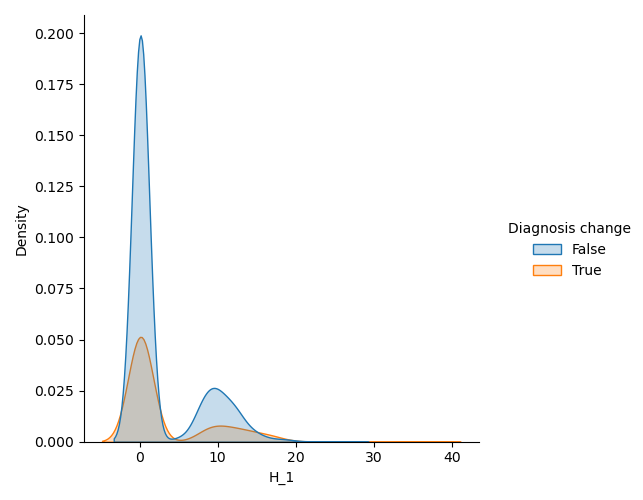
\includegraphics[width=\textwidth]{figures/temporal_evolution/landscape_H_1_dist_diag_change.png}
    \caption{$L^{1}$ landscape distance with 1 layer in $H_1$}
  \end{subfigure}
  \begin{subfigure}{0.32\textwidth}
    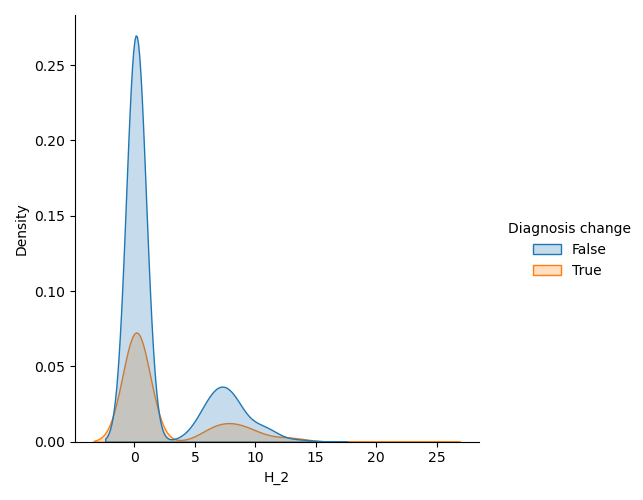
\includegraphics[width=\textwidth]{figures/temporal_evolution/landscape_H_2_dist_diag_change.png}
    \caption{$L^{1}$ landscape distance with 1 layer in $H_2$}
  \end{subfigure}
  \caption{Kernel density estimation of the average average distance between each image timepoint for each patient. The orange curve represents all those patients who have had at least one change in diagnosis over the course of the disease, whereas patients who haven't are within the blue curve.}
  \label{fig:kde_intra_patient}
\end{figure}

\subsection{Topological outliers and misclassified samples.}

The distribution of distances with respect to the average persistent landscape was plotted for the patients who were correctly classified, and for those who were not correctly classified. The results are shown in Figure~\ref{fig:outlier_misclassified}. We also examined the proportion of patients who switched diagnosis in the whole ADNI dataset. We found that 70\% (64) of the misclassified patients had only one diagnosis versus 71\% (323) in the whole dataset.

\begin{figure}
  \centering
  \begin{subfigure}{0.32\textwidth}
    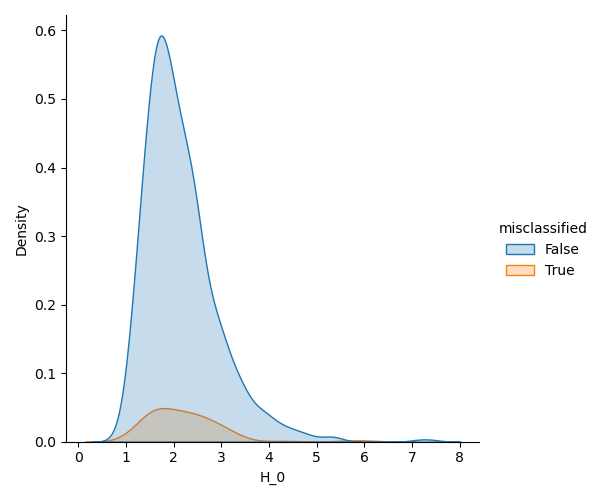
\includegraphics[width=\textwidth]{figures/misclassification_distance/distribution_distance_misclassified_CN_H_0.png}
    \caption{Distance from median CN PL in $H_0$}
  \end{subfigure}
  \begin{subfigure}{0.32\textwidth}
    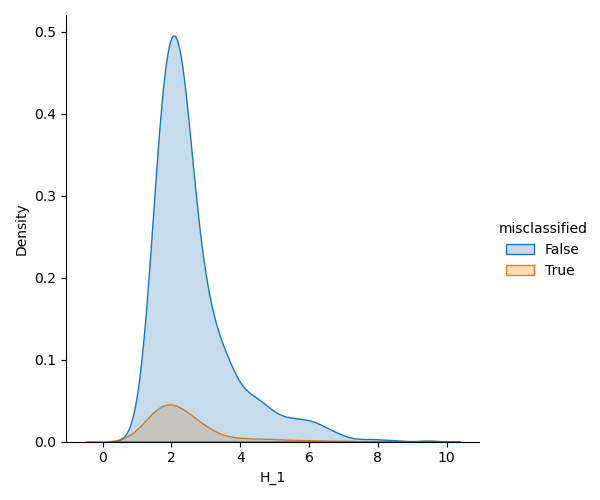
\includegraphics[width=\textwidth]{figures/misclassification_distance/distribution_distance_misclassified_CN_H_1.png}
    \caption{Distance from median CN PL in $H_1$}
  \end{subfigure}
  \begin{subfigure}{0.32\textwidth}
    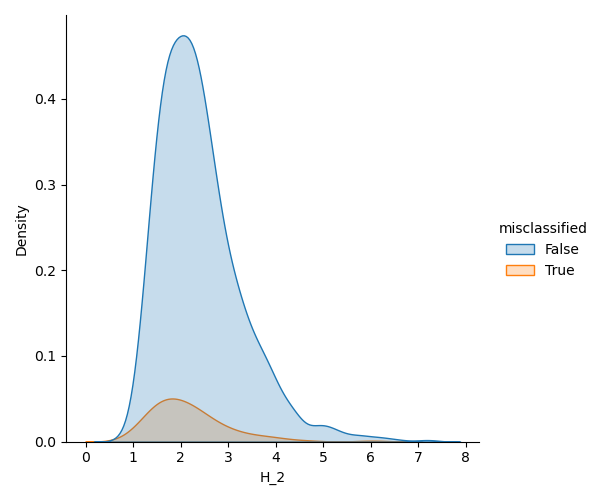
\includegraphics[width=\textwidth]{figures/misclassification_distance/distribution_distance_misclassified_CN_H_2.png}
    \caption{Distance from median CN PL in $H_2$}
  \end{subfigure}
  \begin{subfigure}{0.32\textwidth}
    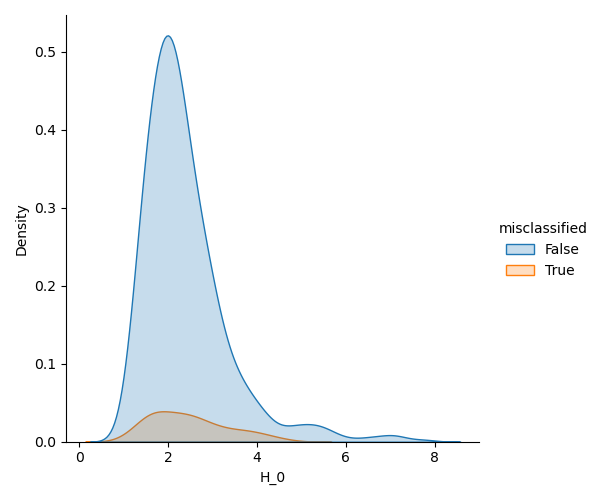
\includegraphics[width=\textwidth]{figures/misclassification_distance/distribution_distance_misclassified_AD_H_0.png}
    \caption{Distance from median AD PL in $H_0$}
  \end{subfigure}
  \begin{subfigure}{0.32\textwidth}
    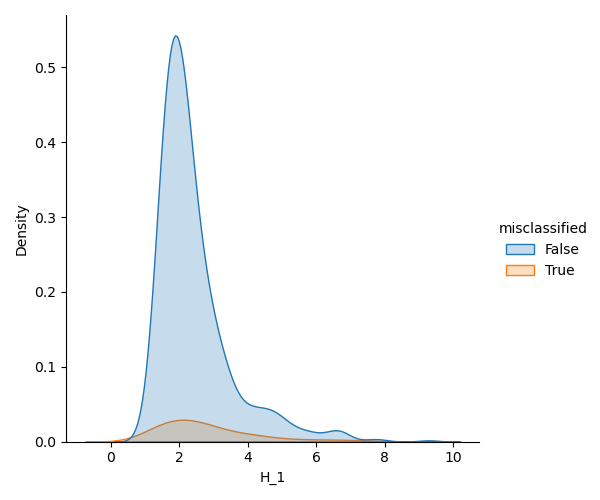
\includegraphics[width=\textwidth]{figures/misclassification_distance/distribution_distance_misclassified_AD_H_1.png}
    \caption{Distance from median AD PL in $H_1$}
  \end{subfigure}
  \begin{subfigure}{0.32\textwidth}
    \includegraphics[width=\textwidth]{figures/misclassification_distance/distribution_distance_misclassified_AD_H_2.png}
    \caption{Distance from median AD PL in $H_2$}
  \end{subfigure}
    \caption{Kernel density estimation of distribution of the distance between the AD and CN median persistence image for images which have and haven't been misclassified.}
  \label{fig:outlier_misclassified}
\end{figure}

\section{Discussion}\label{sec:discussion}

Here, we discuss our findings and their significance. First, we discuss how the qualitative differences in persistence images seen across patients translates to overall competitive classification performance results; we then move onto discuss our findings regarding the distributions of distances among diagnostic categories and within patients. Finally, we outline some limitations and further research avenues to be explored in the future.

\subsection{Persistence images \& classification}

The qualitative differences between the patches observed in Figure ~\ref{fig:sample_rep_pi} do indeed generalize across the dataset; we indeed obtain competitive performance results (shown in Table ~\ref{tab:performance}). While the classification performance is lower to the results reported in \citep{wen2020convolutional} (which are about 80\% to 90\%), our results were obtained using a very simple neural architecture and only the local topological features of a single, small patch in the temporal lobe, which is very encouraging. Further signs showing that our accuracy might be improved is that there is no increased ratio of topological outliers among the misclassified samples (Figure~\ref{fig:outlier_misclassified}), nor is the proportion of patients showing a change in diagnosis substantially higher among misclassified samples, showing that patients who are oscillating between two diagnostic categories do not account for a high uncertainty.

Another source of performance increase would be a multi-patch setup, where the persistent image of other relevant patches could be considered. This stems from the fact that there is increasing evidence for the existence of biological subtypes of AD, and could account for a significant amount of misclassified samples. Evidence for biological subtypes of AD which could also translate in differentially affected brain regions in of AD is emerging \citep{tijms2020pathophysiological,poulakis2018heterogeneous}. In this context, computing the PI of other patches which are affected by other subtypes of AD, like the precuneus, the medial and lateral temporal cortex, some of which incidentally also show increased AUCPRC rates in patch-based classification as seen in Figure ~\ref{fig:aucprc}.

\subsection{Distances}\label{sec:disc-dist}

As shown in Figure \ref{fig:displots_median_pl}, the distribution of the distances of the persistent landscapes of each patch PL to the median PL for each of these diagnostic categories (shown in Figure ~\ref{fig:median_pls}) is very skewed, with some images having high values compared to the rest of the patients (see Table ~\ref{tab:stats_median_pl} and Figure ~\ref{tab:stats_median_pl}). While the overall skew is most pronounced among MCI patients, pointing to a genuinely increased topological heterogeneity within this particular diagnostic category, some of the more extreme values can be attributed to noise introduced at any step of the data acquisition and preprocessing steps described in section \ref{sec:methods}. Note that this phenomenon could also underlie the heterogeneity of the results we see in the comparisons made within a single patient, which we discuss next.

Contrary to expectation, little appreciable difference was seen in intra-patient samples across distance functions, despite seeing significant (at significance threshold $\alpha=0.01$) results from the Mann-Whitney $\mathcal{U}$ test $p$-values for all samples observed in Figure \ref{fig:kde_intra_patient}. The reason for this lack of signal is likely due to the fact that the level of noise introduced by averaging for each patient likely drown any signal. More sensitive clustering techniques using PDs could be more useful to determine the temporal trajectory of each patient. Additionally, the features extracted from a local patch features is enough to characterize global atrophy progression patterns seen in the cortex of Alzheimer's patients over time, as noted elsewhere \citep{toniolo2018patterns}.

\subsection{Limitations and outlook}

The first drawback of our analysis is the difficulty to highlight sources of noise in the features. For instance, we mention in section \ref{sec:disc-dist} that some of the topological outliers that were highlighted in Figure \ref{fig:displots_median_pl} could be due to noise, but the source of that noise is unknown. Specifically, it is not possible to investigate whether this noise comes from the preprocessing pipeline applied to it, or from the latent data distribution. We hypothesize that part of the noise could be introduced during the mapping of the original $T_1$-weighted image to the reference normalized MNI space.

Another overall limitation of the findings presented here is the coarseness of the analyses related to distances. While we wanted to get an insight into the rawest form of the data possible, taking the $L^1$ norm between some vector representations of the persistence diagram for instance, can artificially drown highly discriminatory features. Therefore, the potential of the topological features to discriminate between patients who progress from a baseline diagnosis or not can be further investigated using more advanced clustering techniques making use of the topological features extracted using persistent homology.

More specifically, some coarseness was deliberately introduced by extracting only one layer when analysing persistence landscapes. This value was chosen because we are interested in changes in the highly persistent features of the data, hence eliminating the noise arising from the persistent homology computation. On a similar note, the performance of our classifier could have further be optimized using a deeper and more optimized architecture, but the choice of a simple architecture was made to assess the saliency of the data rather than the potential of the classifier itself to yield good results with little computation.

Finally, our classification task does not cover the full spectrum of all of the possible diagnoses a patient coming to a memory clinic might present. Importantly, our model was not trained to classify patients who have a case of MCI, which is neither AD nor CN, but in between. It is possible that the discriminatory power of the features used in this report might not enable the full fledged classification task required in the clinic. Further studies need to also assess the saliency of the PI obtained from the temporal patch in question for a better assessment of the clinical usefulness of persistent homology in classifying the various categories of patients.

Despite these limitations, it is important to point out that the approach outlined here was specifically aimed at analysing  MRI images obtained from patients with Alzheimer's disease, it could also be applied to any other neurodegenerative disorder. Other prevalent neurodegenerative disorders include Parkinson's disease, dementia with Lewy bodies, and genetically inherited diseases like Huntington's disease, which all have distinct atrophy patterns and, hence, topological signatures. Adaptations would be required, such as adapting the choice of patch of interest -- as an example, it might be more relevant to look at the basal ganglia for Huntington's disease.

Additionally, we note that a clustering using topological descriptors could be used to more finely delineate subtypes of AD and various stages of progression. For instance, using deep clustering techniques and embeddings using persistence images as inputs could yield useful insights into the various stages of progression and subtypes of dementia. These more sensitive methods could then, once fine-tuned, hopefully also track preclinical stages of AD, when atrophy is present but does not results in cognitive decline due to the presence of a cognitive reserve \citep{scarmeas2004cognitive, van2017neuroimaging}. The identification of patient populations at risk of developing the disease could then form the target of any potential preventive treatment.

\section{Conclusion}

In this report we have shown that PIs computed from a patch in the temporal lobe are salient for classifying CN and AD subjects. Additionally, we show that the distribution of distances among the patients in each of the diagnostic category is skewed, indicating the presence of topological outliers, but, overall, does not affect the classification performance. Finally, we show a significant, but not substantial, increase in distance among images belonging to a given patient who deteriorates towards Alzheimer's disease versus patients who do not. Although promising, all of these topology-driven approaches need further development to maximize the information that can be extracted from MRI images.

\clearpage
\bibliographystyle{unsrtnat}
\bibliography{main}

\clearpage
\appendix

\section{Supplements}
\subsection{Preprocessing of MRI data}\label{apd:preprocessing}
We included all T1-weighted MRI images from ADNI1, 2, 3, and GO, which were captured and preprocessed by ADNI.
Results included in our work come from preprocessing performed using \texttt{fMRIPrep} 20.1.1, a Nipype 1.5.0 based tool.
All MRIs were corrected for intensity non-uniformity (INU) with \texttt{N4BiasFieldCorrection}, distributed with ANTs 2.2.0, and used as T1w-reference throughout the workflow.
The T1w-reference was then skull-stripped with a \texttt{Nipype} implementation of
the \texttt{antsBrainExtraction.sh} workflow (from ANTs), using \texttt{OASIS30ANTs} as a target template.
%Brain tissue segmentation of cerebrospinal fluid (CSF),
%white-matter (WM) and gray-matter (GM) was performed on
%the brain-extracted T1w using `fast` [FSL 5.0.7]. %, RRID:SCR_002823, @fsl_fast].
Volume-based spatial normalisation to a standard coordinate space~(\texttt{MNI152NLin2009cAsym}) was performed through
nonlinear registration with \texttt{antsRegistration}, using brain-extracted versions of both T1w reference and the T1w template.
We slected the template `ICMB 152 Nonlinear Asymmetrical Template Version 2009c' for spatial normalisation.
% [@mni152nlin2009casym, RRID:SCR_008796; TemplateFlow ID: MNI152NLin2009cAsym],

Many internal operations of \texttt{fMRIPrep} use the
\texttt{Nilearn} library, version 0.6.2, % [@nilearn, RRID:SCR_001362],
mostly within the functional processing workflow.
For more details of the pipeline, please refer to \href{https://fMRIPrep.readthedocs.io/en/latest/workflows.html}{the official documentation of \texttt{fMRIPrep}}. Preprocessing was finalised by intensity normalisation of the extracted and MNI space registered brain images. %[the section corresponding to workflows in *fMRIPrep*'s documentation](https://fMRIPrep.readthedocs.io/en/latest/workflows.html "fMRIPrep's documentation").



\end{document}
